\documentclass[../main.tex]{subfiles}

\usepackage{nopageno} %Seitenzahlen auf richtiger Seite 

\usepackage[left=2cm, right=2cm, top=2cm, includehead, includefoot, headheight=17pt]{geometry}

\usepackage[utf8x]{inputenc}
\usepackage[english]{babel}
\usepackage{amsmath,amssymb,amsthm}
\usepackage{framed}
\usepackage{wasysym}
\usepackage[T1]{fontenc} %Silbentrennung 
\usepackage{color} %Farbe
\usepackage{graphicx}
\usepackage{float}%Grafik am gleichen Ort plazieren
%pdf. png. einfach eingliedern
\usepackage{subfigure} %Grafiken nebeneinander
\usepackage{pdfpages}
\usepackage{ulem} 	%\uuline{urgent}    % doppelt unterstreichen
%\uwave{boat}      % unterschlängeln
%\sout{wrong}       % durchstreichen
%\xout{removed}     % ausstreichen mit //////.

\usepackage{tikz}
\usetikzlibrary{trees}
\usetikzlibrary{plotmarks}
\usetikzlibrary{angles,quotes,babel}
\usetikzlibrary{shadings}
\usetikzlibrary{patterns}
\usetikzlibrary{matrix}
\usetikzlibrary{arrows}
\usetikzlibrary{calc}

\usepackage{pgfplots}
\usepackage{pgf-pie}
\pgfplotsset{compat=1.10}
\usepgfplotslibrary{statistics}
\usepgfplotslibrary{fillbetween}

\usepackage{tkz-euclide}
\usepackage{enumerate}
\usepackage{stmaryrd}
\usepackage{tabularx}
\usepackage{wrapfig}
\usepackage{epsdice}
\usepackage{multirow}
\usepackage{rotating}
\usepackage{pdflscape}
\usepackage{fancyhdr}

\pagestyle{fancy} %eigener Seitenstil
\fancyhf{} %alle Kopf- und Fußzeilenfelder bereinigen
\fancyhead[L]{} %Kopfzeile links
\fancyhead[C]{} %zentrierte Kopfzeile
\fancyhead[R]{} %Kopfzeile rechts
\renewcommand{\headrulewidth}{0.4pt} %obere Trennlinie
\fancyfoot[C]{\thepage} %Seitennummer
\renewcommand{\footrulewidth}{0.4pt} %untere Trennlinie

% Number spaces 
\newcommand{\CC}{\ensuremath{\mathbb{C}}}
\newcommand{\RR}{\ensuremath{\mathbb{R}}}
\newcommand{\QQ}{\ensuremath{\mathbb{Q}}}
\newcommand{\ZZ}{\ensuremath{\mathbb{Z}}}
\newcommand{\NN}{\ensuremath{\mathbb{N}}}
\newcommand{\LL}{\ensuremath{\mathbb{L}}}
\newcommand{\DD}{\ensuremath{\mathbb{D}}}
\newcommand{\WW}{\ensuremath{\mathbb{W}}}

%draw chemestry molecules 
\usepackage{chemfig} % https://mirror.ox.ac.uk/sites/ctan.org/macros/generic/chemfig/

\newcommand\vv[1]{%
	\begin{tikzpicture}[baseline=(arg.base)]
		\node[inner xsep=0pt] (arg) {$#1$};
		\draw[line cap=round,line width=0.45,->,shorten >= 0.2pt, shorten <= 0.7pt] (arg.north west) -- (arg.north east);
	\end{tikzpicture}%
} %command will render \vv{x} with an arrow aboth 

\renewcommand{\labelenumi}{\roman{enumi})}

\DeclareMathOperator{\ggT}{ggT}
\DeclareMathOperator{\sign}{sign}

%sections
\theoremstyle{plain}
\newtheorem{Thm}{Theorem}[section]
\newtheorem{Def}[Thm]{Definition}
\newtheorem{Prop}[Thm]{Proposition}

\theoremstyle{definition}
\newtheorem{lemma}[Thm]{Lemma}
\newtheorem{corollary}[Thm]{Corollary}
\newtheorem{claim}[Thm]{Claim}
\newtheorem{Proof}[Thm]{Proof}
\newtheorem{Ex}[Thm]{Example}

\newtheorem{Exercise}{ex}[section] %follow proper enum
\newtheorem{ex}[Exercise]{Exercise}
\newtheorem{Solution}{sol}[section]
\newtheorem{sol}[Solution]{Solution}

\theoremstyle{remark}
\newtheorem{remark}[Thm]{Remark} % follows thm enum

\newtheorem{comment}{Comment}[section] %follow comment enum
\newtheorem{notation}[comment]{Notation}
\newtheorem{reasoning}[comment]{Reasoning}
\newtheorem{Intpr}[comment]{Interpretation}

%some premmade with title (uterwise use \textbf{Title} ...)
\newenvironment{ThmWithTitle}[1]{%
	\begin{Thm}[\textbf{#1}]}{\end{Thm}}
\newenvironment{PropWithTitle}[1]{%
	\begin{Prop}[\textbf{#1}]}{\end{Prop}}
\newenvironment{ExWithTitle}[1]{%
	\begin{Ex}[\textbf{#1}]}{\end{Ex}}
\newenvironment{DefWithTitle}[1]{%
	\begin{Def}[\textbf{#1}]}{\end{Def}}
\newenvironment{RemarkWithTitel}[1]{%
	\begin{remark}[\textbf{#1}]}{\end{remark}}

%format of paragraph 
\renewcommand\paragraph{\@startsection{paragraph}{4}{\z@}%
	{-2.5ex\@plus -1ex \@minus -.25ex}%
	{1.25ex \@plus .25ex}%
	{\normalfont\normalsize\bfseries}}
\makeatother
\setcounter{secnumdepth}{4} % how many sectioning levels to assign numbers to
\setcounter{tocdepth}{4}    % how many sectioning levels to show in ToC

\newcounter{row} 
\renewcommand\therow{\alph{row}} %hier a,b,c etc. def und mit therow abrufbar

\newenvironment{aufz}
{\setcounter{row}{0}%
	\par\noindent\tabularx{\linewidth}[t]
	{\cdot{20}{>{\stepcounter{row}\makebox[1.5em][l]{\therow)\hfill}}X}} %bis max 20 Elemente nebeinander
}
{\endtabularx}


%biblio
\usepackage[]{biblatex}
\addbibresource{referenzenma.bib} 

%glossary
\usepackage{glossaries}
\usepackage{import}


\usepackage{rotating} % Include this package in the preamble

%\newglossaryentry{Enzyme}{
	name={Enzyme},
	description={A macromolecular biological catalyst that significantly accelerates chemical reactions, often with high specificity. They can be proteins or catalytically active RNA molecules:contentReference[oaicite:0]{index=0}.}
}

\newglossaryentry{Cofactor}{
	name={Cofactor},
	description={An inorganic chemical component required for enzyme activity. Often metal ions such as Fe\textsuperscript{2+}, Mg\textsuperscript{2+}, or Zn\textsuperscript{2+}:contentReference[oaicite:1]{index=1}.}
}

\newglossaryentry{Coenzyme}{
	name={Coenzyme},
	description={A complex organic or metallorganic molecule required for enzyme function, often derived from vitamins. Acts as a transient carrier of specific functional groups:contentReference[oaicite:2]{index=2}.}
}

\newglossaryentry{Systematic name}{
	name={Systematic name},
	description={A precise name given to an enzyme that indicates the substrates and type of reaction it catalyzes (e.g., ATP:glucose phosphotransferase for hexokinase):contentReference[oaicite:3]{index=3}.}
}

\newglossaryentry{Classification number}{
	name={Classification number},
	description={A four-part code assigned to enzymes based on the type of reaction they catalyze (e.g., 2.7.1.1 for hexokinase):contentReference[oaicite:4]{index=4}.}
}

\newglossaryentry{Activation Energy}{
	name={Activation Energy},
	description={The energy barrier ($$\Delta G^{\ddagger}$$) between the ground state and the transition state that must be overcome for a reaction to proceed:contentReference[oaicite:5]{index=5}.}
}

\newglossaryentry{Transition State Theory}{
	name={Transition State Theory},
	description={A model describing the top of the energy hill in a reaction coordinate where reactants are equally likely to proceed to products or return to reactants. Not to be confused with reaction intermediates:contentReference[oaicite:6]{index=6}.}
}

\newglossaryentry{Transition State}{
	name={Transition State},
	description={The highest-energy configuration along the reaction coordinate. It is the point at which the system is equally likely to proceed toward products or return to reactants. It is not a stable intermediate and is denoted as $\ddagger$:contentReference[oaicite:0]{index=0}.}
}


\newglossaryentry{Reaction Intermediate}{
	name={Reaction Intermediate},
	description={A short-lived, chemically distinct species that occurs during the transformation of reactants to products, such as enzyme-substrate (ES) complexes:contentReference[oaicite:7]{index=7}.}
}

\newglossaryentry{K_{eq}}{
	name={$K_{eq}$},
	description={The equilibrium constant of a reaction, given by the ratio $$\frac{[P]}{[S]}$$. Not affected by enzymes:contentReference[oaicite:8]{index=8}.}
}

\newglossaryentry{Delta G}{
	name={$\Delta G$},
	description={The change in free energy during a reaction. $\Delta G°$ refers to standard conditions, and $\Delta G°^{\prime}$ includes biochemical conditions (pH = 7):contentReference[oaicite:9]{index=9}.}
}

\newglossaryentry{Delta G dagger}{
	name={$\Delta$ $G^{\ddagger}$},
	description={The activation free energy, the difference in energy between the ground state and the transition state:contentReference[oaicite:10]{index=10}.}
}

\newglossaryentry{Return Rate}{
	name={Return Rate},
	description={The rate of the reaction based on substrate concentration and a rate constant $$k$$, where $$v = k[S]$$:contentReference[oaicite:11]{index=11}.}
}

\newglossaryentry{Catalytic Power}{
	name={Catalytic Power},
	description={The ability of enzymes to lower the activation energy and provide alternate reaction pathways, enhancing the reaction rate:contentReference[oaicite:12]{index=12}.}
}

\newglossaryentry{Active Site}{
	name={Active Site},
	description={The region of the enzyme where substrate binding and catalysis occur, often through specific amino acid residues:contentReference[oaicite:13]{index=13}.}
}

\newglossaryentry{Transition State Complementarity}{
	name={Transition State Complementarity},
	description={The enzyme binds more tightly to the transition state than to the substrate, thereby lowering the activation energy and enhancing catalysis:contentReference[oaicite:14]{index=14}.}
}

\newglossaryentry{Rate Enhancement}{
	name={Rate Enhancement},
	description={The increase in reaction speed due to the lowering of the activation energy by enzyme catalysis:contentReference[oaicite:15]{index=15}.}
}

\newglossaryentry{Binding}{
	name={Binding},
	description={The specific interaction between enzyme and substrate, often involving multiple weak noncovalent interactions to drive catalysis:contentReference[oaicite:16]{index=16}.}
}

\newglossaryentry{Specificity}{
	name={Specificity},
	description={The enzyme's ability to select exact substrates and catalyze a specific reaction, influenced by binding energy and structural complementarity:contentReference[oaicite:17]{index=17}.}
}

\newglossaryentry{Acid-Base Catalysis}{
	name={Acid-Base Catalysis},
	description={A catalytic mechanism in which amino acid residues act as proton donors or acceptors to stabilize charged intermediates, increasing reaction rates when water alone is insufficient:contentReference[oaicite:0]{index=0}.}
}

\newglossaryentry{Covalent Catalysis}{
	name={Covalent Catalysis},
	description={A mechanism where the enzyme forms a transient covalent bond with the substrate, creating an alternative reaction pathway with lower activation energy. This requires nucleophilic groups on the enzyme:contentReference[oaicite:1]{index=1}.}
}

\newglossaryentry{Metal Ion Catalysis}{
	name={Metal Ion Catalysis},
	description={Catalysis involving metal ions that can stabilize negative charges on reaction intermediates, help substrate orientation, or mediate redox reactions through reversible changes in oxidation state:contentReference[oaicite:2]{index=2}.}
}

\newglossaryentry{Enzyme Kinetics}{
	name={Enzyme Kinetics},
	description={The study of the rate of enzyme-catalyzed reactions and how they change in response to experimental parameters like substrate concentration:contentReference[oaicite:3]{index=3}.}
}

\newglossaryentry{v_0}{
	name={$v_0$},
	description={The initial velocity of an enzyme-catalyzed reaction, measured at the very beginning before product accumulates. At low $[S]$, $v_0$ increases almost linearly with $[S]$:contentReference[oaicite:4]{index=4}.}
}

\newglossaryentry{Enzyme Saturation}{
	name={Enzyme Saturation},
	description={The condition where increasing substrate concentration no longer increases the reaction rate because all active sites are occupied, resulting in a plateau at $v_{max}$:contentReference[oaicite:5]{index=5}.}
}

\newglossaryentry{v_{max}}{
	name={$v_{max}$},
	description={The maximal velocity of an enzyme-catalyzed reaction when all enzyme molecules are saturated with substrate. Defined by $v_{max} = k_{cat}[E]_T$:contentReference[oaicite:6]{index=6}.}
}

\newglossaryentry{Michaelis-Menten}{
	name={Michaelis-Menten},
	description={A kinetic model describing enzyme activity: $v_0 = \frac{v_{max}[S]}{K_m + [S]}$, where $K_m$ is the substrate concentration at half-maximal velocity:contentReference[oaicite:7]{index=7}.}
}

\newglossaryentry{Lineweaver-Burk}{
	name={Lineweaver-Burk},
	description={A double reciprocal plot of enzyme kinetics: $\frac{1}{v_0} = \frac{K_m}{v_{max}} \cdot \frac{1}{[S]} + \frac{1}{v_{max}}$, used to linearize the Michaelis-Menten equation for easier interpretation:contentReference[oaicite:8]{index=8}.}
}

\newglossaryentry{Enzyme Efficiency}{
	name={Enzyme Efficiency},
	description={Measured by the specificity constant $\frac{k_{cat}}{K_m}$, which reflects both substrate binding and catalytic turnover. The theoretical upper limit is $10^8$ to $10^9 \text{ M}^{-1}\text{s}^{-1}$:contentReference[oaicite:9]{index=9}.}
}

\newglossaryentry{Inhibition}{
	name={Inhibition},
	description={The decrease or complete loss of enzyme activity due to the binding of a molecule (an inhibitor) that interferes with catalysis. Inhibition is fundamental to drug action and metabolic regulation:contentReference[oaicite:0]{index=0}.}
}

\newglossaryentry{Reversible Inhibition}{
	name={Reversible Inhibition},
	description={Inhibition where the inhibitor binds non-covalently and can dissociate from the enzyme. Includes competitive, non-competitive, and uncompetitive mechanisms:contentReference[oaicite:1]{index=1}.}
}

\newglossaryentry{Competitive Inhibitor}{
	name={Competitive Inhibitor},
	description={A molecule that competes with the substrate for binding at the active site. It increases $K_m$ but does not affect $v_{max}$:contentReference[oaicite:2]{index=2}.}
}

\newglossaryentry{Non-competitive Inhibitor}{
	name={Non-competitive Inhibitor},
	description={Binds to a site other than the active site and reduces the effective concentration of active enzyme. It decreases $v_{max}$ without changing $K_m$:contentReference[oaicite:3]{index=3}.}
}

\newglossaryentry{Uncompetitive Inhibitor}{
	name={Uncompetitive Inhibitor},
	description={Binds only to the enzyme-substrate complex, preventing product formation. It decreases both $v_{max}$ and $K_m$:contentReference[oaicite:4]{index=4}.}
}

\newglossaryentry{Irreversible Inhibition}{
	name={Irreversible Inhibition},
	description={Inhibition where the inhibitor covalently binds or permanently inactivates the enzyme, preventing further catalytic activity:contentReference[oaicite:5]{index=5}.}
}

\newglossaryentry{Suicide Inhibition}{
	name={Suicide Inhibition},
	description={A special type of irreversible inhibition where the enzyme converts the inhibitor into a reactive intermediate that covalently modifies and inactivates the enzyme:contentReference[oaicite:6]{index=6}.}
}

\newglossaryentry{Transition-State Analogs}{
	name={Transition-State Analogs},
	description={Stable molecules that resemble the transition state of a substrate and bind tightly to the enzyme, acting as potent inhibitors by exploiting transition state complementarity:contentReference[oaicite:7]{index=7}.}
}




\makeglossaries
\newglossaryentry{Enzyme}{
	name={Enzyme},
	description={A macromolecular biological catalyst that significantly accelerates chemical reactions, often with high specificity. They can be proteins or catalytically active RNA molecules:contentReference[oaicite:0]{index=0}.}
}

\newglossaryentry{Cofactor}{
	name={Cofactor},
	description={An inorganic chemical component required for enzyme activity. Often metal ions such as Fe\textsuperscript{2+}, Mg\textsuperscript{2+}, or Zn\textsuperscript{2+}:contentReference[oaicite:1]{index=1}.}
}

\newglossaryentry{Coenzyme}{
	name={Coenzyme},
	description={A complex organic or metallorganic molecule required for enzyme function, often derived from vitamins. Acts as a transient carrier of specific functional groups:contentReference[oaicite:2]{index=2}.}
}

\newglossaryentry{Systematic name}{
	name={Systematic name},
	description={A precise name given to an enzyme that indicates the substrates and type of reaction it catalyzes (e.g., ATP:glucose phosphotransferase for hexokinase):contentReference[oaicite:3]{index=3}.}
}

\newglossaryentry{Classification number}{
	name={Classification number},
	description={A four-part code assigned to enzymes based on the type of reaction they catalyze (e.g., 2.7.1.1 for hexokinase):contentReference[oaicite:4]{index=4}.}
}

\newglossaryentry{Activation Energy}{
	name={Activation Energy},
	description={The energy barrier ($$\Delta G^{\ddagger}$$) between the ground state and the transition state that must be overcome for a reaction to proceed:contentReference[oaicite:5]{index=5}.}
}

\newglossaryentry{Transition State Theory}{
	name={Transition State Theory},
	description={A model describing the top of the energy hill in a reaction coordinate where reactants are equally likely to proceed to products or return to reactants. Not to be confused with reaction intermediates:contentReference[oaicite:6]{index=6}.}
}

\newglossaryentry{Transition State}{
	name={Transition State},
	description={The highest-energy configuration along the reaction coordinate. It is the point at which the system is equally likely to proceed toward products or return to reactants. It is not a stable intermediate and is denoted as $\ddagger$:contentReference[oaicite:0]{index=0}.}
}


\newglossaryentry{Reaction Intermediate}{
	name={Reaction Intermediate},
	description={A short-lived, chemically distinct species that occurs during the transformation of reactants to products, such as enzyme-substrate (ES) complexes:contentReference[oaicite:7]{index=7}.}
}

\newglossaryentry{K_{eq}}{
	name={$K_{eq}$},
	description={The equilibrium constant of a reaction, given by the ratio $$\frac{[P]}{[S]}$$. Not affected by enzymes:contentReference[oaicite:8]{index=8}.}
}

\newglossaryentry{Delta G}{
	name={$\Delta G$},
	description={The change in free energy during a reaction. $\Delta G°$ refers to standard conditions, and $\Delta G°^{\prime}$ includes biochemical conditions (pH = 7):contentReference[oaicite:9]{index=9}.}
}

\newglossaryentry{Delta G dagger}{
	name={$\Delta$ $G^{\ddagger}$},
	description={The activation free energy, the difference in energy between the ground state and the transition state:contentReference[oaicite:10]{index=10}.}
}

\newglossaryentry{Return Rate}{
	name={Return Rate},
	description={The rate of the reaction based on substrate concentration and a rate constant $$k$$, where $$v = k[S]$$:contentReference[oaicite:11]{index=11}.}
}

\newglossaryentry{Catalytic Power}{
	name={Catalytic Power},
	description={The ability of enzymes to lower the activation energy and provide alternate reaction pathways, enhancing the reaction rate:contentReference[oaicite:12]{index=12}.}
}

\newglossaryentry{Active Site}{
	name={Active Site},
	description={The region of the enzyme where substrate binding and catalysis occur, often through specific amino acid residues:contentReference[oaicite:13]{index=13}.}
}

\newglossaryentry{Transition State Complementarity}{
	name={Transition State Complementarity},
	description={The enzyme binds more tightly to the transition state than to the substrate, thereby lowering the activation energy and enhancing catalysis:contentReference[oaicite:14]{index=14}.}
}

\newglossaryentry{Rate Enhancement}{
	name={Rate Enhancement},
	description={The increase in reaction speed due to the lowering of the activation energy by enzyme catalysis:contentReference[oaicite:15]{index=15}.}
}

\newglossaryentry{Binding}{
	name={Binding},
	description={The specific interaction between enzyme and substrate, often involving multiple weak noncovalent interactions to drive catalysis:contentReference[oaicite:16]{index=16}.}
}

\newglossaryentry{Specificity}{
	name={Specificity},
	description={The enzyme's ability to select exact substrates and catalyze a specific reaction, influenced by binding energy and structural complementarity:contentReference[oaicite:17]{index=17}.}
}

\newglossaryentry{Acid-Base Catalysis}{
	name={Acid-Base Catalysis},
	description={A catalytic mechanism in which amino acid residues act as proton donors or acceptors to stabilize charged intermediates, increasing reaction rates when water alone is insufficient:contentReference[oaicite:0]{index=0}.}
}

\newglossaryentry{Covalent Catalysis}{
	name={Covalent Catalysis},
	description={A mechanism where the enzyme forms a transient covalent bond with the substrate, creating an alternative reaction pathway with lower activation energy. This requires nucleophilic groups on the enzyme:contentReference[oaicite:1]{index=1}.}
}

\newglossaryentry{Metal Ion Catalysis}{
	name={Metal Ion Catalysis},
	description={Catalysis involving metal ions that can stabilize negative charges on reaction intermediates, help substrate orientation, or mediate redox reactions through reversible changes in oxidation state:contentReference[oaicite:2]{index=2}.}
}

\newglossaryentry{Enzyme Kinetics}{
	name={Enzyme Kinetics},
	description={The study of the rate of enzyme-catalyzed reactions and how they change in response to experimental parameters like substrate concentration:contentReference[oaicite:3]{index=3}.}
}

\newglossaryentry{v_0}{
	name={$v_0$},
	description={The initial velocity of an enzyme-catalyzed reaction, measured at the very beginning before product accumulates. At low $[S]$, $v_0$ increases almost linearly with $[S]$:contentReference[oaicite:4]{index=4}.}
}

\newglossaryentry{Enzyme Saturation}{
	name={Enzyme Saturation},
	description={The condition where increasing substrate concentration no longer increases the reaction rate because all active sites are occupied, resulting in a plateau at $v_{max}$:contentReference[oaicite:5]{index=5}.}
}

\newglossaryentry{v_{max}}{
	name={$v_{max}$},
	description={The maximal velocity of an enzyme-catalyzed reaction when all enzyme molecules are saturated with substrate. Defined by $v_{max} = k_{cat}[E]_T$:contentReference[oaicite:6]{index=6}.}
}

\newglossaryentry{Michaelis-Menten}{
	name={Michaelis-Menten},
	description={A kinetic model describing enzyme activity: $v_0 = \frac{v_{max}[S]}{K_m + [S]}$, where $K_m$ is the substrate concentration at half-maximal velocity:contentReference[oaicite:7]{index=7}.}
}

\newglossaryentry{Lineweaver-Burk}{
	name={Lineweaver-Burk},
	description={A double reciprocal plot of enzyme kinetics: $\frac{1}{v_0} = \frac{K_m}{v_{max}} \cdot \frac{1}{[S]} + \frac{1}{v_{max}}$, used to linearize the Michaelis-Menten equation for easier interpretation:contentReference[oaicite:8]{index=8}.}
}

\newglossaryentry{Enzyme Efficiency}{
	name={Enzyme Efficiency},
	description={Measured by the specificity constant $\frac{k_{cat}}{K_m}$, which reflects both substrate binding and catalytic turnover. The theoretical upper limit is $10^8$ to $10^9 \text{ M}^{-1}\text{s}^{-1}$:contentReference[oaicite:9]{index=9}.}
}

\newglossaryentry{Inhibition}{
	name={Inhibition},
	description={The decrease or complete loss of enzyme activity due to the binding of a molecule (an inhibitor) that interferes with catalysis. Inhibition is fundamental to drug action and metabolic regulation:contentReference[oaicite:0]{index=0}.}
}

\newglossaryentry{Reversible Inhibition}{
	name={Reversible Inhibition},
	description={Inhibition where the inhibitor binds non-covalently and can dissociate from the enzyme. Includes competitive, non-competitive, and uncompetitive mechanisms:contentReference[oaicite:1]{index=1}.}
}

\newglossaryentry{Competitive Inhibitor}{
	name={Competitive Inhibitor},
	description={A molecule that competes with the substrate for binding at the active site. It increases $K_m$ but does not affect $v_{max}$:contentReference[oaicite:2]{index=2}.}
}

\newglossaryentry{Non-competitive Inhibitor}{
	name={Non-competitive Inhibitor},
	description={Binds to a site other than the active site and reduces the effective concentration of active enzyme. It decreases $v_{max}$ without changing $K_m$:contentReference[oaicite:3]{index=3}.}
}

\newglossaryentry{Uncompetitive Inhibitor}{
	name={Uncompetitive Inhibitor},
	description={Binds only to the enzyme-substrate complex, preventing product formation. It decreases both $v_{max}$ and $K_m$:contentReference[oaicite:4]{index=4}.}
}

\newglossaryentry{Irreversible Inhibition}{
	name={Irreversible Inhibition},
	description={Inhibition where the inhibitor covalently binds or permanently inactivates the enzyme, preventing further catalytic activity:contentReference[oaicite:5]{index=5}.}
}

\newglossaryentry{Suicide Inhibition}{
	name={Suicide Inhibition},
	description={A special type of irreversible inhibition where the enzyme converts the inhibitor into a reactive intermediate that covalently modifies and inactivates the enzyme:contentReference[oaicite:6]{index=6}.}
}

\newglossaryentry{Transition-State Analogs}{
	name={Transition-State Analogs},
	description={Stable molecules that resemble the transition state of a substrate and bind tightly to the enzyme, acting as potent inhibitors by exploiting transition state complementarity:contentReference[oaicite:7]{index=7}.}
}



\begin{document}
	


\section{Cell Signaling: Principles}

\subsubsection{The Basic Vocabulary of Cell Signaling}

\begin{figure}[h]
	\centering
	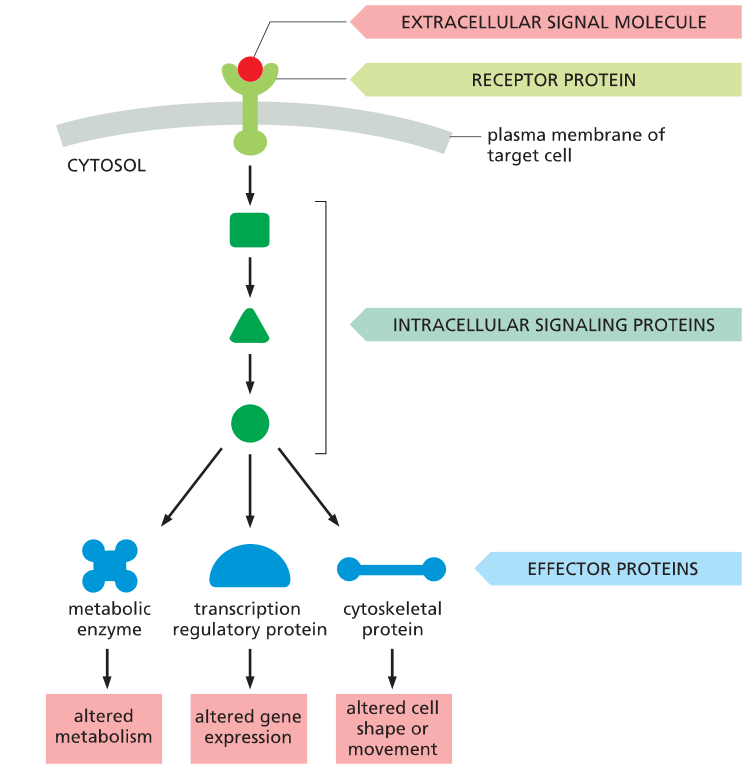
\includegraphics[width=0.45\textwidth]{Basic_overview}
	\caption{Basic Vocabulary of Cell Signaling}
\end{figure}

There are some key terms in \gls{CellSignaling}. Here's a run down of how they connect in cell signaling:
\begin{enumerate}
	\item An \textbf{\gls{ExtracellularSignalingMolecule}} binds to a \textbf{signal receiving protein or receptor}.
	\item That \gls{Receptor} is generally a transmembrane protein but can also be intracellular. This receptor is activated through the binding (generally some sort of conformational change).
	\item This causes a \textbf{\gls{Signalingcascade}} through a chain of \textbf{intracellular signaling proteins} activating each other, usually branching out.
	\item The final protein in that cascade will then change the activity of the \gls{Effectorproteins}, which launches the cellular response.
	\item These \textbf{effector proteins} can be metabolic enzymes, transcription regulators, or cytoskeletal proteins.
\end{enumerate}

\subsubsection{Cell-surface vs. Intracellular Receptors}

There are two main differences between Cell-Surface and Intracellular receptors:

First, the location of the receptors (surprised you with that am I right):
\begin{itemize}
	\item \gls{CellSurfaceReceptor}: generally transmembrane protein, where the signaling molecule binds extracellularly.
	\item \gls{IntracellularReceptor}: The receptor protein will be close or even inside the nucleus.
\end{itemize}

Then, accordingly the signaling molecule will also be different, in the case of:
\begin{itemize}
	\item Cell-Surface, it is generally a \textbf{hydrophilic} signaling molecule. This means the molecule can't enter the cell, so we need the receptor to have some extracellular component.
	\item Intracellular, it is a small \textbf{hydrophilic} signaling molecule, which can transfer the cell membrane. This is necessary as it needs to reach the receptor in the nucleus. They are carrier through the blood by carrier proteins (hydrophilic).
\end{itemize}


\subsubsection{The Four Subtypes of Cell Signaling and Two Variations}

\begin{figure}[H]
	\centering
	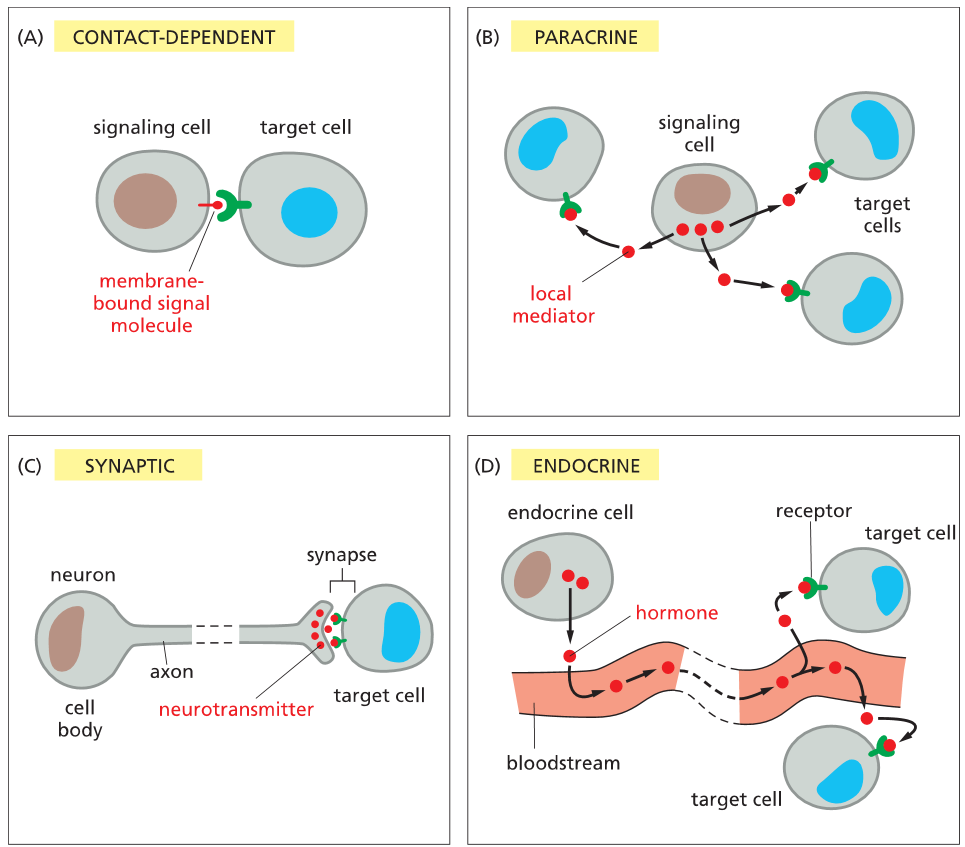
\includegraphics[width=0.45\textwidth]{4_horsemen}
	\caption{The Four types of Signaling}
\end{figure}

\textbf{\gls{ContactDependentSignaling}}:
\begin{itemize}
	\item Area of signal: Cells are in contact.
	\item Form of communication: Proteins which are attached to the cells interact. One protein serves as the signal and the other as receptor.
	\item Variation: the cell can also have contact dependent interactions with the extracellular matrix (e.g., collagen), for more details see section on ECM.
\end{itemize}


\textbf{\gls{ParacrineSignaling}}:
\begin{itemize}
	\item Area of signal: Cells are not in contact. This is usually a local signal, just a few cells away.
	\item Form of communication: One protein secreted by a cell, is the signal or ligand and attaches to the receptor of a different cell.
\end{itemize}


\textbf{\gls{SynapticSignaling}}:
\begin{itemize}
	\item Area of signal: Cells are not in contact. Small distance between releaser of ligand and receptor, called the synapse. Very local signal.
	\item Form of communication: Secretion of a ligand or \gls{Neurotransmitter}. Released by one cell and recepted by another.
\end{itemize}


\textbf{\gls{EndocrineSignaling,hormonalsignaling} a.k.a. hormonal signaling}:
\begin{itemize}
	\item Area of signal: Cells are not in contact. Can be long distance and have effects from anywhere to anywhere
	\item Form of communication: A hormone is produced by cell A and then released into the bloodstream, where it can then leave at some point and serve as a signal to a receptor protein.
\end{itemize}

\begin{DefWithTitle}{\gls{AutocrineSignaling}}
	If a cell receives its own signal it is called autocrine signaling.
\end{DefWithTitle}

\begin{DefWithTitle}{\gls{ConstitutivelyActive}}
	A protein (usually a receptor or enzyme) that is always active, regardless of whether it has received a signal or a ligand is bounded. This can lead to uncontrolled signaling and is often seen in cancer. The reason for this is generally a mutation to the gene of the protein. 
\end{DefWithTitle}

\subsubsection{The diversity in Signals}

\textbf{The same signal can cause a multitude of signals}. This section will have a look of the consequences and opportunities of that. 

\textbf{Multiple signaling molecules}, better the combination can cause very different signals: Depending on the combination of signals received a cell can kill, proliferate, or differentiate itself. Further the same signaling ligand or protein can have very different consequences depending on the receptor or cell it attaches to. See for example acetylcholine: 

\begin{figure}[H]
	\centering
	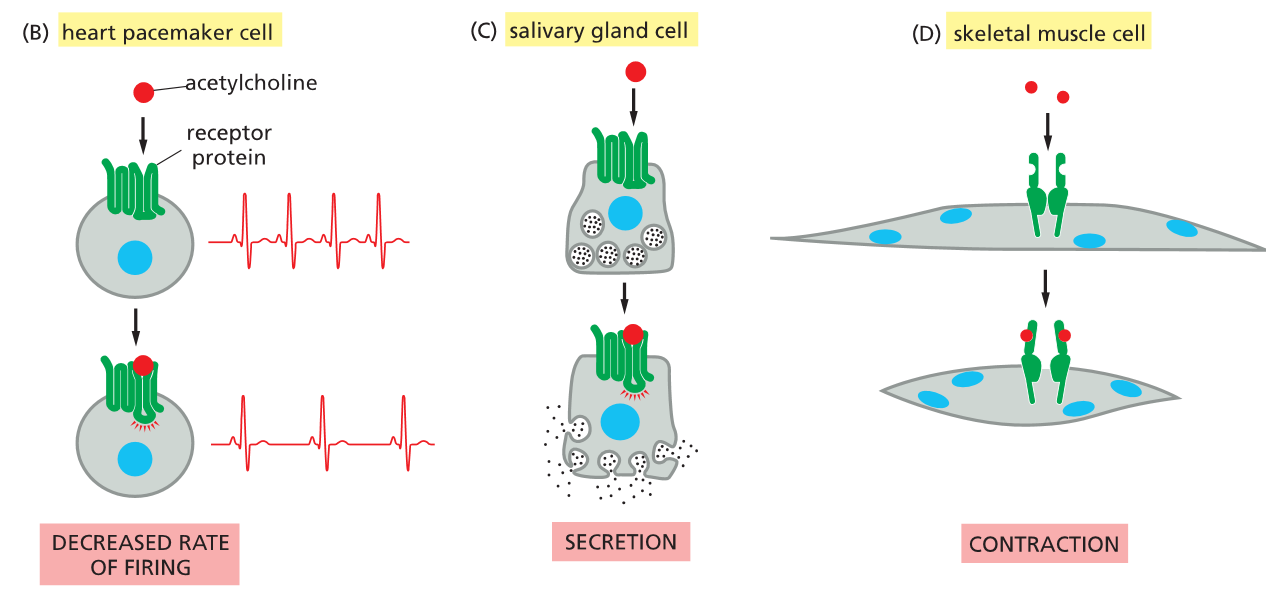
\includegraphics[width=0.6\textwidth]{Acetylcholine}
	\caption{Examples of Acetylcholine having vastly different responses to its signal.}
\end{figure}

\textbf{Speed of the response}: Depending on the response path, the response by the cell can be fast or slow. If the response alters a protein it will take seconds to minutes, while if the gene has to be transcribed it takes minutes to hours. These two types are called \textbf{\gls{ProteinResponse}} or \textbf{\gls{Transcriptionalresponse}}. Some receptors also cause both the fast and slow response path. 

\begin{figure}[H]
	\centering
	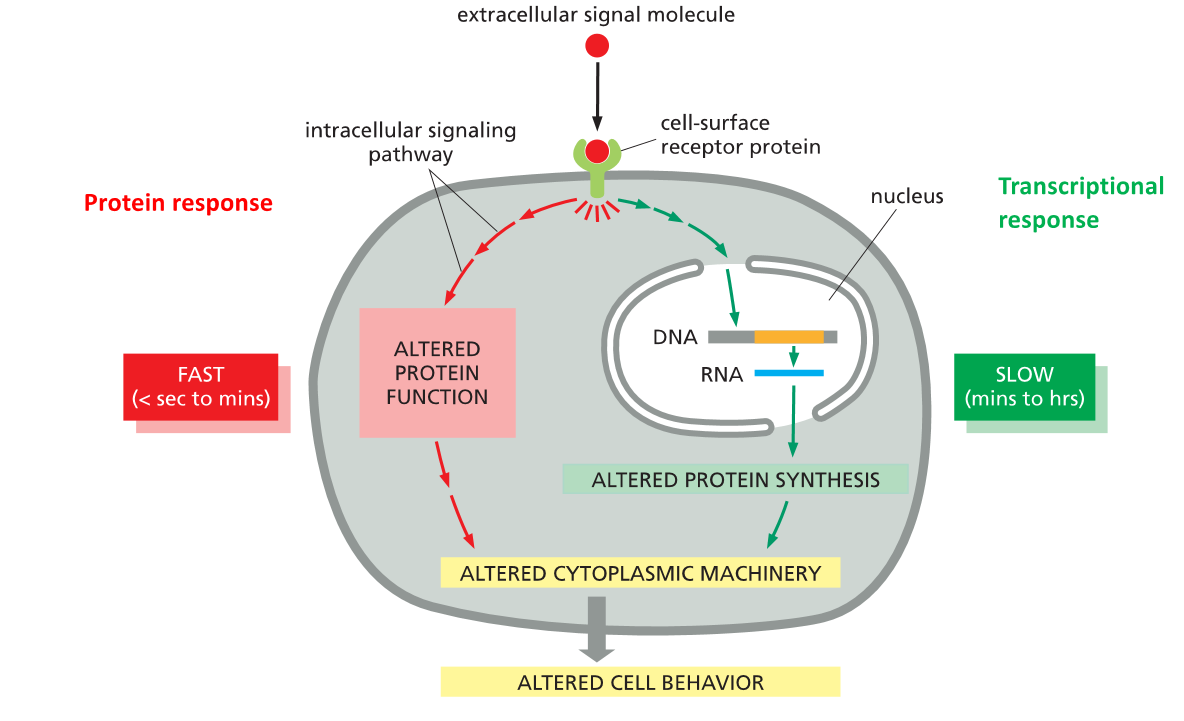
\includegraphics[width=0.6\textwidth]{response_speed}
	\caption{An overview of protein (fast) vs. transcriptional (slow) response.}
\end{figure}

Examples of a fast response: change in movement, secretion, or metabolism, caused by e.g., phosphorylation. Concretely the recruitment of GLUT transporters from recycling endosomes, has to occur very rapidly once insulin docks onto the receptor.

\begin{figure}[H]
	\centering
	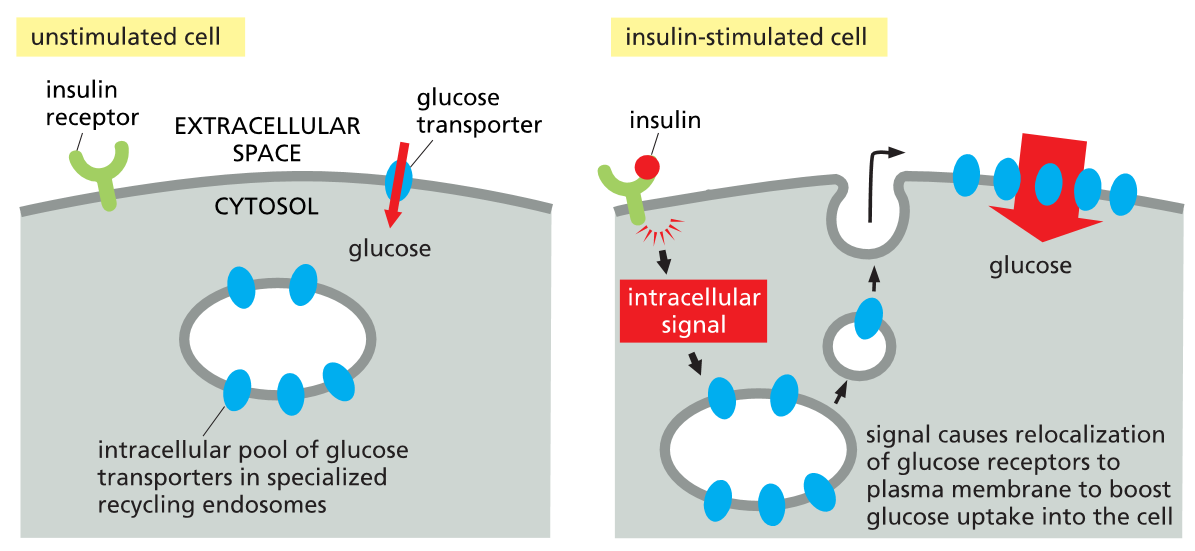
\includegraphics[width=0.45\textwidth]{GLUT_fast}
	\caption{An example of a fast protein response with the GLUT transporter.}
\end{figure}

\subsubsection{Classes of Cell-Surface Receptors}

There are three main classes of cell-surface receptors, which we will all be diving into later on:
\begin{enumerate}
	\item \gls{Ion-channel-coupledreceptors} a.k.a. transmitter-gated ion channels;
	\item \gls{G-protein-coupledreceptors};
	\item \gls{Enzymecoupledreceptors};
\end{enumerate}

\begin{figure}[h]
	\centering
	\subfigure[Ion class]{
		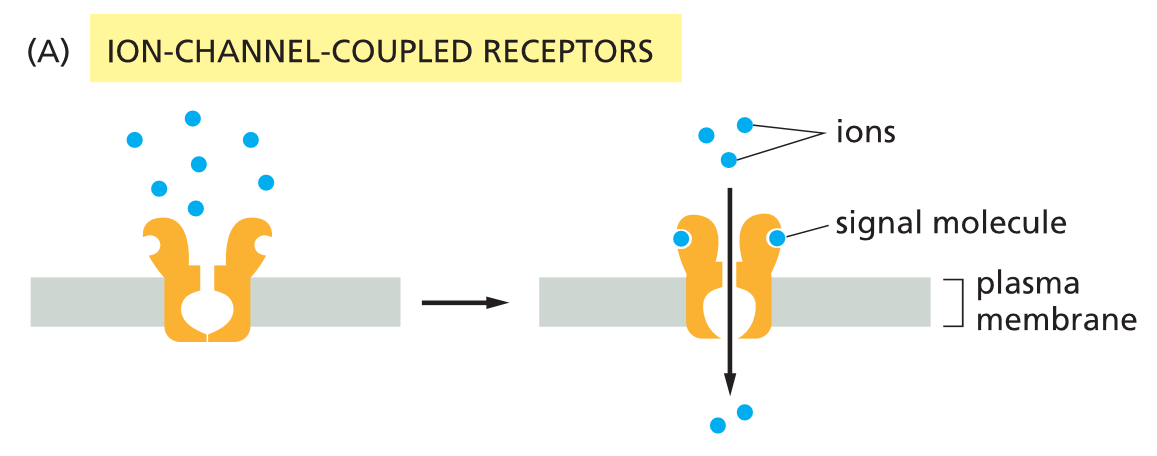
\includegraphics[width=0.45\textwidth]{ion_class}
	}
	\hfill
	% Second subfigure
	\subfigure[G class]{
		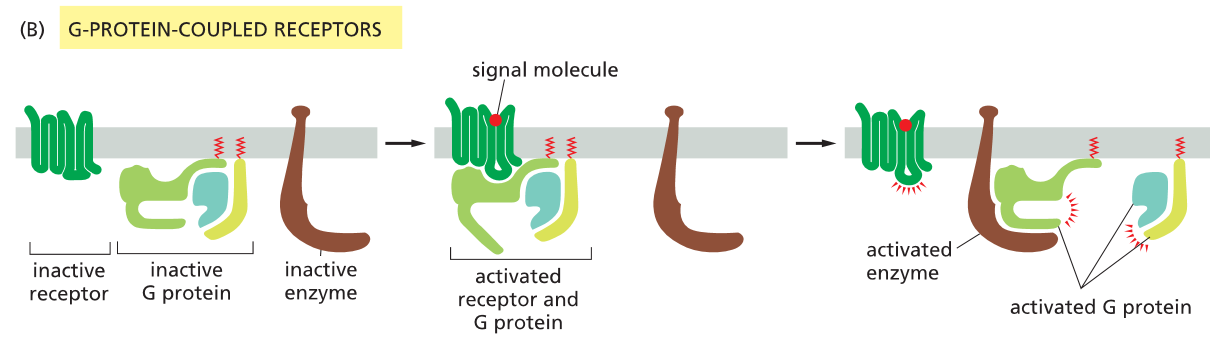
\includegraphics[width=0.5\textwidth]{g_class}
	}
		\hfill
	% Second subfigure
	\subfigure[Enzyme class]{
		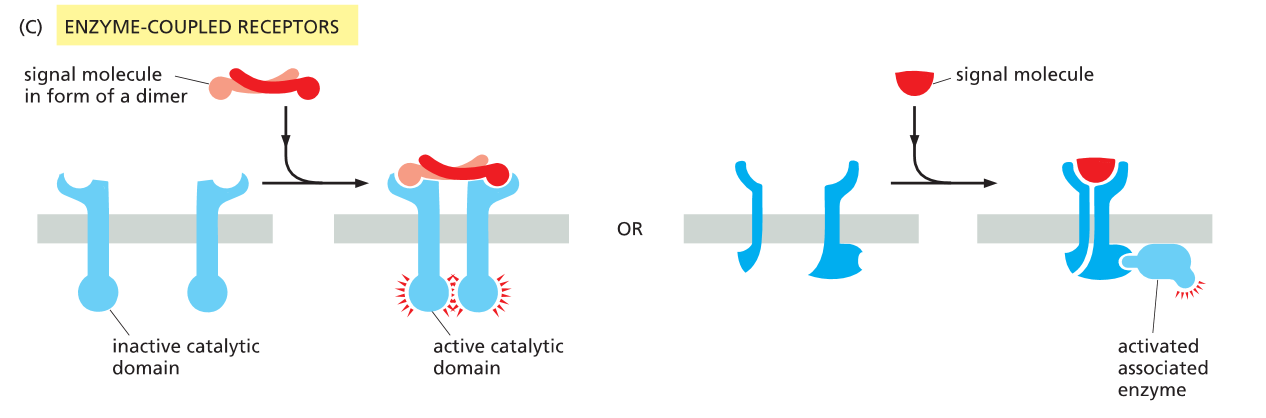
\includegraphics[width=0.5\textwidth]{enzyme_class}
	}
	\caption{The three classes of cell-surface receptors}
\end{figure}
Note on the enzyme-coupled one: There are two options here: one where the enzyme is part of the receptor and another where the enzyme is recruited. Ligands activate the receptors by promoting their dimerization though, regardless if the enzyme is directly attached or not.

\subsubsection{Regulation of Intracellular Signaling Proteins}
\label{sec:GTP}

There are two main \textbf{\gls{Molecularswitches}} for intracellular signaling proteins:
\begin{enumerate}
	\item \textbf{\gls{Phosphorylation}} 
	\begin{itemize}
		\item based on a phosphate group being attached to the protein (attached means active).
		\item phosphorylation or dephosphorylation often leads to change in formation and to activation.
		\item Addition by kinases.
		\item Removal by phosphatases.
		\item This group can be added to three amino acids: Tyrosine, Threonine, or Serine. This is because they have an alcohol which works for the attack on the phosphate.
	\end{itemize}
	\item \textbf{\gls{GTPbinding}}
	\begin{itemize}
		\item  \textbf{\gls{GTPases}} are molecular switches that cycle between active (GTP-bound) and inactive (GDP-bound) states. This is also a type of G-Protein, but a different class of monomeric "small" GTPases.
		\item A phosphate is removed from GTP to make GDP, this deactivates the molecule. GDP stays bound.
		\item With an incoming signal, this GDP can be exchanged for a GTP.
		\item \textbf{\gls{GEF}} activate GTPases, by exchanging GDP for GTP.
		\item \textbf{\gls{GAP}s} inactivate GTPases by hydrolyzing GTP and yes GAP stands for GTPase-activating protein, as it activates the inactivation.
		\item Since the cell has a ratio of 10:1 for GTP:GDP, the exchange of GDP to GTP is very favorable.
	\end{itemize}
\end{enumerate}
	
\begin{figure}[h]
	\centering
	\subfigure[Phosphorylation as molecular switch]{
		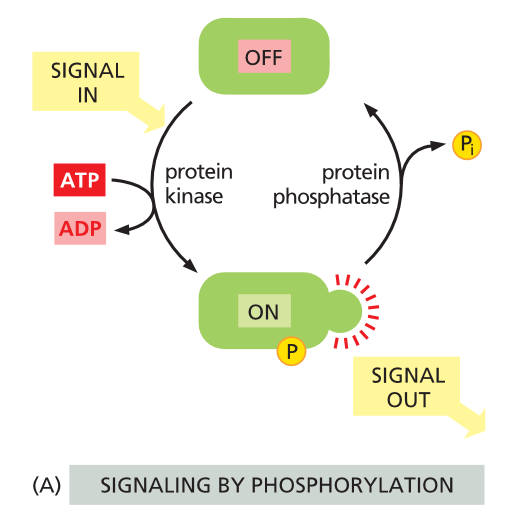
\includegraphics[width=0.45\textwidth]{intra_phospy}
	}
	\hfill
	% Second subfigure
	\subfigure[GTP as molecular switch]{
		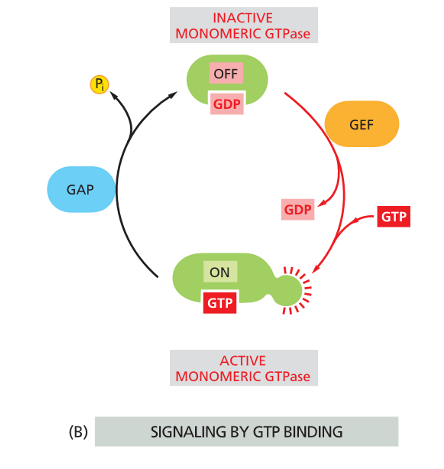
\includegraphics[width=0.5\textwidth]{intra_GTP}
	}
	\caption{Two types of molecular switches in intracellular signaling}
\end{figure}
 


\subsubsection{Inhibitory Signals as Activators}

Signal transduction isn't always a positive signal, sometimes a \textbf{\gls{Inhibitorysignals}} can lead to activation. Basically the idea is to \textbf{inhibit the inhibitor}.
\begin{figure}[H]
	\centering
	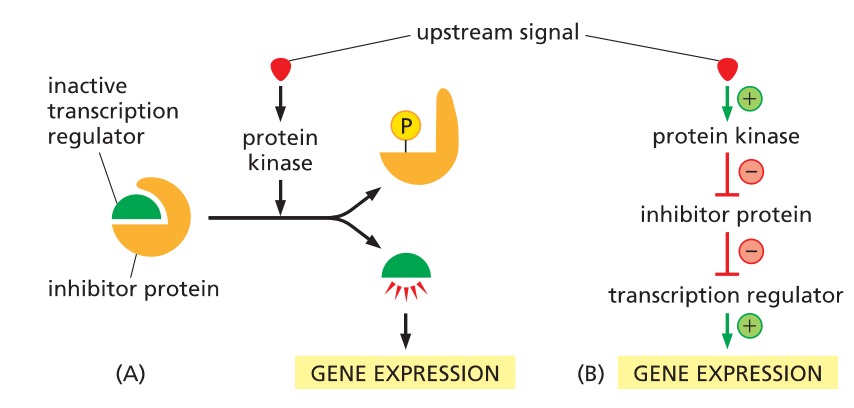
\includegraphics[width=0.6\textwidth]{inhib_ex}
	\caption{Example pathway of an inhibitory signal leads to activation. Note that the left and right path show the same pathway. }
\end{figure}

\subsubsection{Initiating the Signal}

A signal starts through a protein being in \textbf{close proximity} to the signaling compound. This proximity is key and the minimum for a signal to start, additionally ATP can also be required.

There are three main types of starts to signaling (see figure \ref{threesignals}):
\begin{enumerate}
	\item \textbf{Preassembled signaling complex}
	\begin{itemize}
		\item The signal complex is already assembled with all its intracellular signaling proteins, generally in the form of a \textbf{\gls{Scaffoldingprotein}}.
	\end{itemize}
	\item\textbf{\gls{ProteinRecruitment}}
	\begin{itemize}
		\item the signaling proteins are in close proximity. Once the the signal molcule attaches they attach to the receptor.
		\item For the signal to be activated, the signaling proteins don't always need to be physically attached, but just being in close proximity is enough.
	\end{itemize}
	\item \textbf{\gls{Lipidrecruitment}}
	\begin{itemize}
		\item Instead of having the signaling proteins attach to the receptor they attach to a Phosphoinositides (PI, a type of phospholipid). PIs are part of the membrane, in close proximity to the receptor
		\item These phospholipids can be phosphorylated in the cell, which them allows the signaling proteins to attach.
	\end{itemize}
\end{enumerate}

\begin{figure}[H]
	\centering
	\subfigure[Preassembled complex]{
		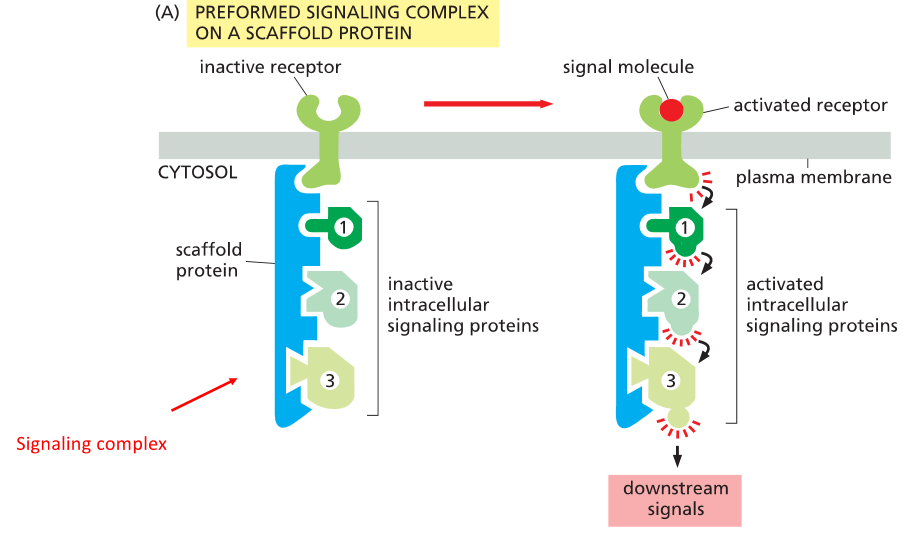
\includegraphics[width=0.45\textwidth]{start_pre}
	}
	\hfill
	% Second subfigure
	\subfigure[Protein recruitment]{
		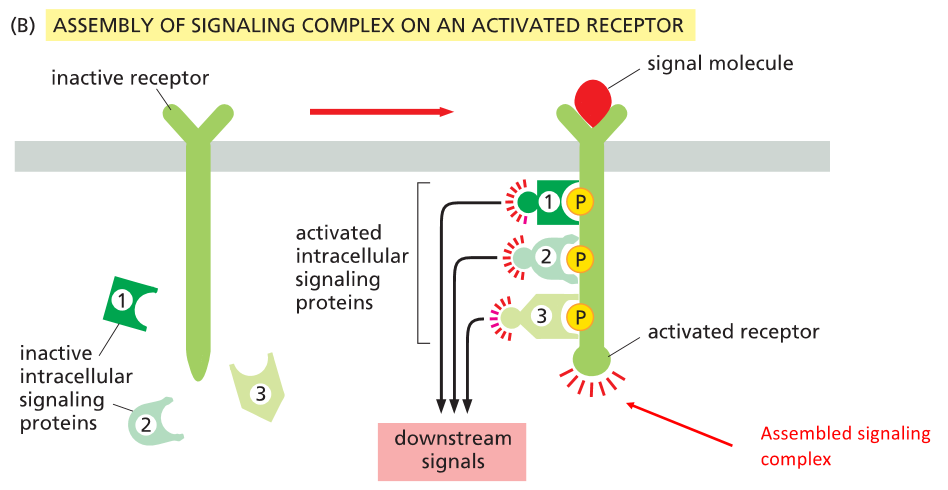
\includegraphics[width=0.5\textwidth]{start_protein}
	}
	\hfill
	% Second subfigure
	\subfigure[Lipid recruitment]{
		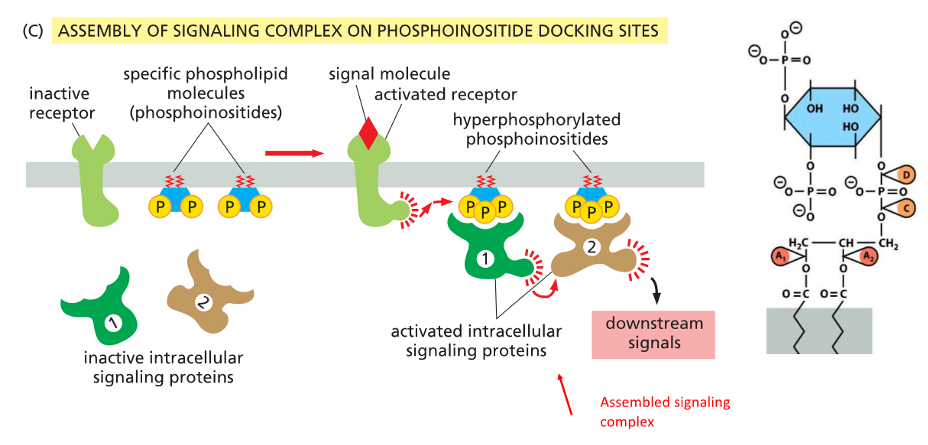
\includegraphics[width=0.5\textwidth]{start_lipid}
	}
	\caption{The three classes of cell-surface receptors}
	\label{threesignals}
\end{figure}

These signaling complex's got their name because they can get very complex. They are formed using \textbf{\gls{ModularInteractionDomain}}. Here is an example of an insulin receptor:

\begin{figure}[H]
	\centering
	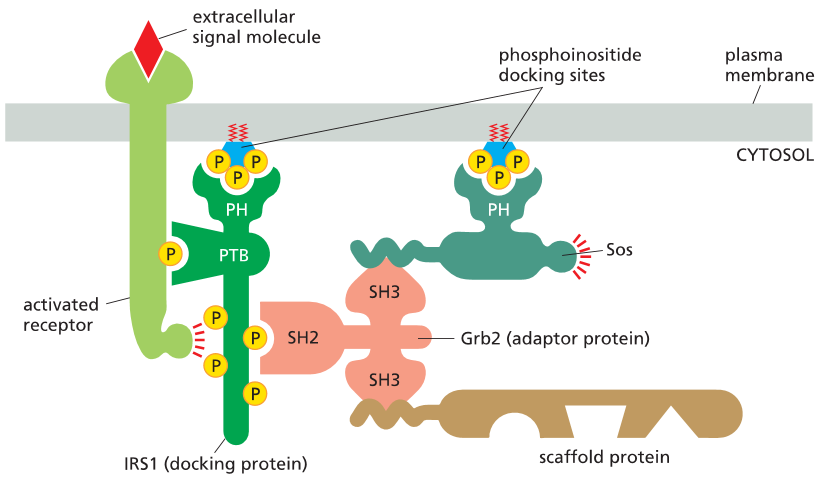
\includegraphics[width=0.45\textwidth]{start_ins}
	\caption{insulin signaling complex as an example for the complexity and modularity of a signaling complex.}
	\label(){startins}
\end{figure}
The shortcuts of the molecules in the figure \ref{startins}:
\begin{itemize}
	\item PH = \textbf{\gls{PleckstrinHomology(PH)}} - binds to phosphorylated PI's
	\item PTB = \textbf{\gls{PhosphotyrosineBinding(PTB)}} - binds phosphotyrosine
	\item SH = \textbf{\gls{SrcHomology(SH)}}, Src is on the first signaling proteins identified in a viral induced chicken sarcoma.
	\item IRS = \textbf{\gls{InsulinReceptorSubstrate(IRS)}}
\end{itemize}


\subsubsection{Regulating and Dampening the Signal}

One way a cell can add extra regulation to a pathway is to require multiple independent pathways to integrate for them to signal downstream, called \textbf{\gls{SignalIntegration}}.
\begin{figure}[H]
	\centering
	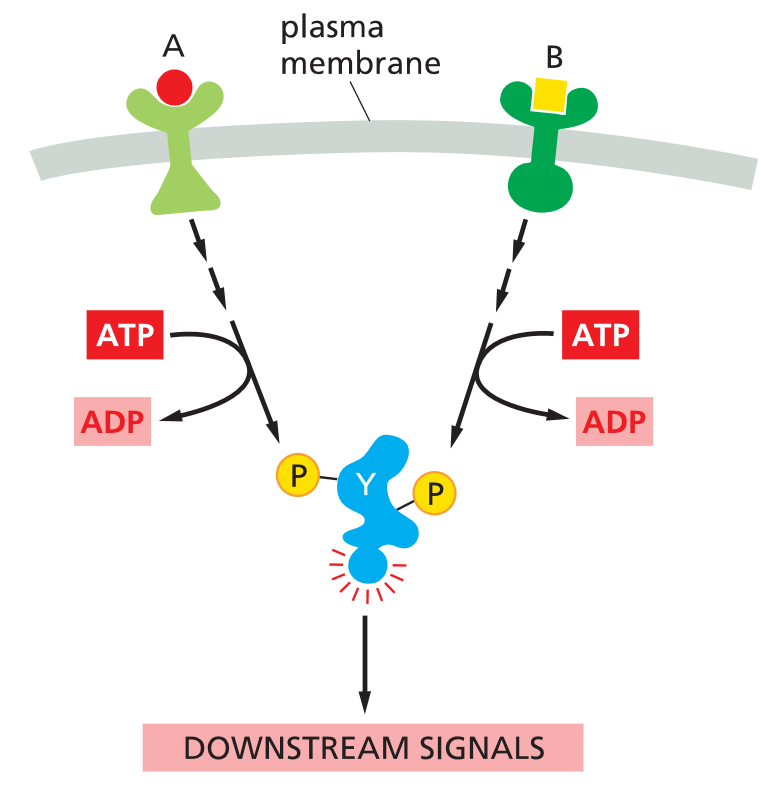
\includegraphics[width=0.45\textwidth]{reg_int}
	\caption{An example pathway showing how multiple streams need to come together to allow downstream signaling.}
\end{figure}

Now, this need for multiple proteins gives the cell the power to change the response duration and strength depending on how it changes the production and degradation rate of each protein. 

\begin{figure}[H]
	\centering
	\subfigure[Equal half life and production (responsive)]{
		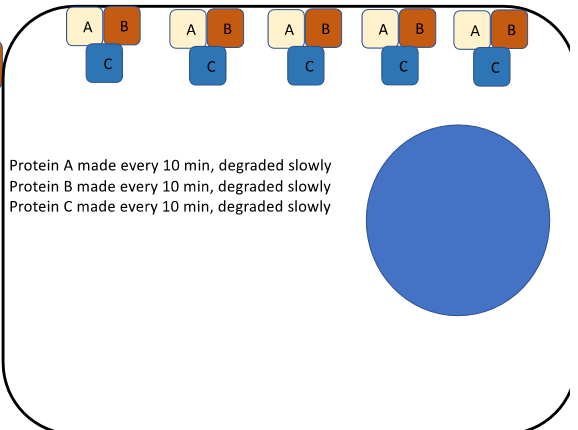
\includegraphics[width=0.3\textwidth]{reg_nor}
	}
	\hfill
	% Second subfigure
	\subfigure[shorter half life, same production (possibly unresponsive)]{
		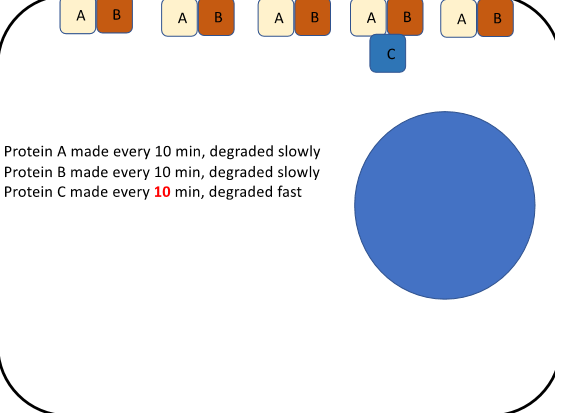
\includegraphics[width=0.3\textwidth]{reg_deg}
	}
	\hfill
	% Second subfigure
	\subfigure[shorter half life and faster production (responsive)]{
		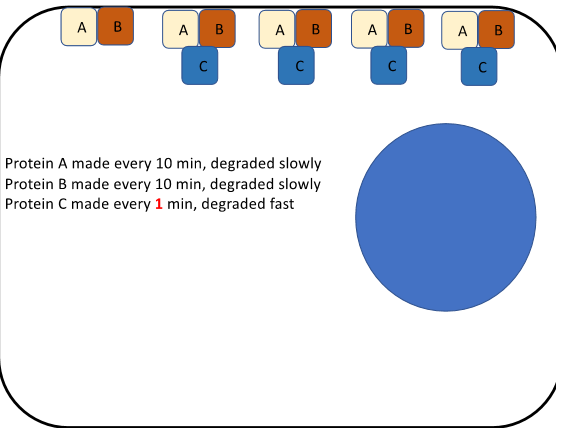
\includegraphics[width=0.3\textwidth]{reg_prod}
	}
	\caption{An example of how influencing the half life and production of certain proteins can seriously influence the responsiveness of a protein complex.}
	\label(){halflife}
\end{figure}

To further show the role and importance of degradation in protein complexes here are some graphs: 
\begin{figure}[H]
	\centering
	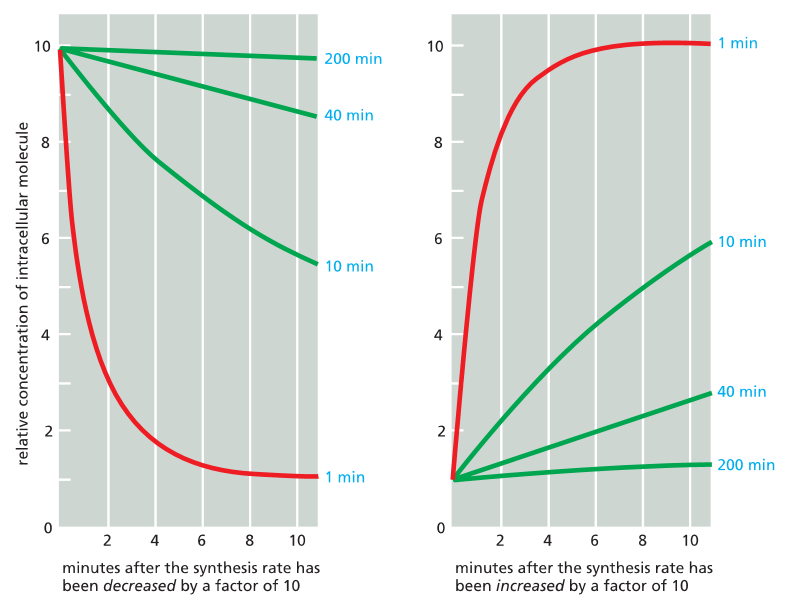
\includegraphics[width=0.45\textwidth]{reg_graph}
	\caption{Shows the connection between \gls{HalfLife} (blue time) and the synthesis rate. The x-axis is the time after the synthesis rate is increased by a factor 10, the y-axis the concentration of the intracellular molecule. A protein with a short half-life will probably also have a high production rate (red line) as otherwise it will be unresponsive (see fig: \ref{halflife}). Hence it will react much more strongly to a signal than a protein with a long half-life and slow production rate (green line).}
\end{figure}



The next key concept is \textbf{\gls{PositiveFeedback} and \gls{NegativeFeedback}}. This is when a downstream molecule will signal upwards in the pathway to either increase or decrease its activity.
\begin{figure}[H]
	\centering
	\subfigure[Shows both positive and negative feedback.]{
		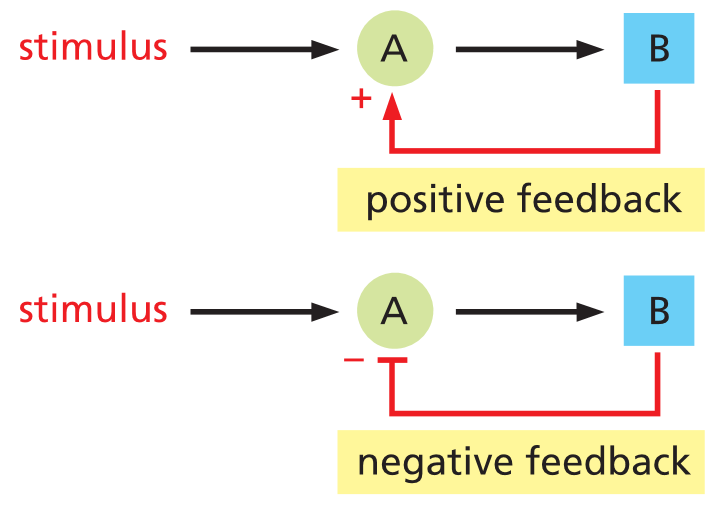
\includegraphics[width=0.3\textwidth]{reg_feed}
	}
	\subfigure[Shows both a positive and negative feedback loop and corresponding time vs. enzyme activity graph.]{
		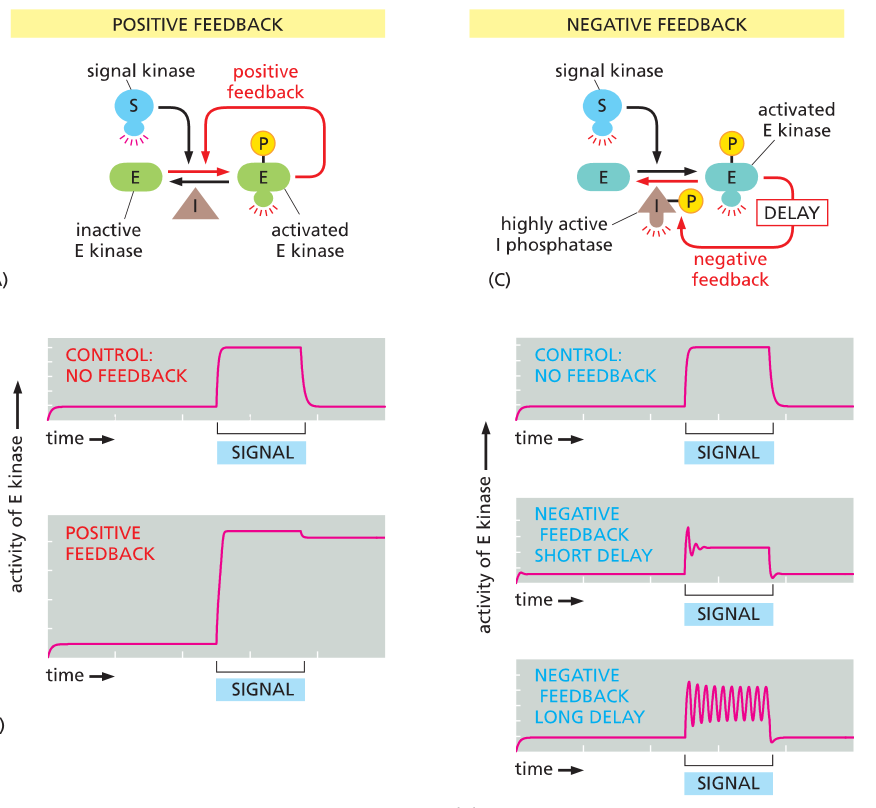
\includegraphics[width=0.65\textwidth]{reg_delay}
	}
	\label{feedback}
\end{figure}

Discussion of the fig: \ref{feedback}: in feedback the positive one is pretty straightforward. You add positive feedback the signal gets extended. For negative feedback the type of delay which is in effect plays a major role, as the dampening gets stronger the more is being produced upstream. So, the reaction is stronger there more upstream there is.
\begin{itemize}
	\item \gls{Shortfeedbackdelay}: in this case after a short pretty strong response it finds a stable dampened state pretty quickly.
	\item \gls{Longfeedbackdelay}: here the signal becomes strong, meanign we get a strong but delayed feedback reaction, once that feedback hits, it kills the signal too strongly, so the feedback gets turned back really strongly. That again allows the signal to become strong and we start over again. \\
\end{itemize}

Next up is \textbf{adapting the extracellular signal molecule}. This will lead to the desensitization or sensitization of the signal molecule. This happens mainly by messing around with the receptor protein, it's quantity and function. It is often done through phosphorylation or ubiquitylation of the receptor proteins. Some are also cases of feedback:

\begin{figure}[H]
	\centering
	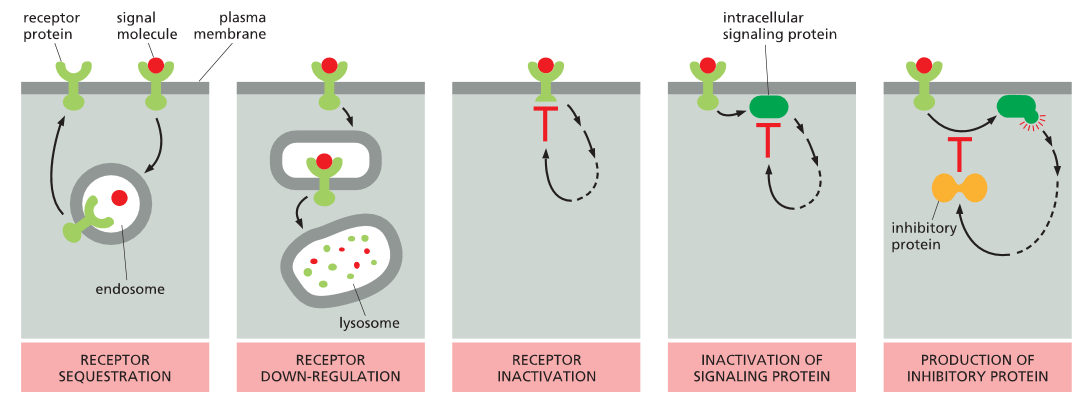
\includegraphics[width=0.8\textwidth]{reg_ext}
	\caption{A bunch of ways the extracellular signal molecule's strength on the pathway can be adapted. This happens mainly by messing around with the receptor protein, it's quantity and function.}
\end{figure}

\subsubsection{All or nothing, Hyperbolic, Sigmoidal Signals}

There are three main shapes a signal response will take on: 
\begin{itemize}
	\item \textbf{\gls{Hyperbolicsignal}}: a gradually increasing cell response to a gradually increasing signal, eventually reaching a plateau.
	\item \textbf{\gls{SigmoidalSignal}}: it takes a while for the signal to take effect, but then results in a steeper reaction at some intermediate concentration
	\item \textbf{\gls{Allornothingsignal}}: extreme form; nothing happens until a certain concentration threshold is reached and then we get a full signal.
\end{itemize}
\begin{figure}[H]
	\centering
	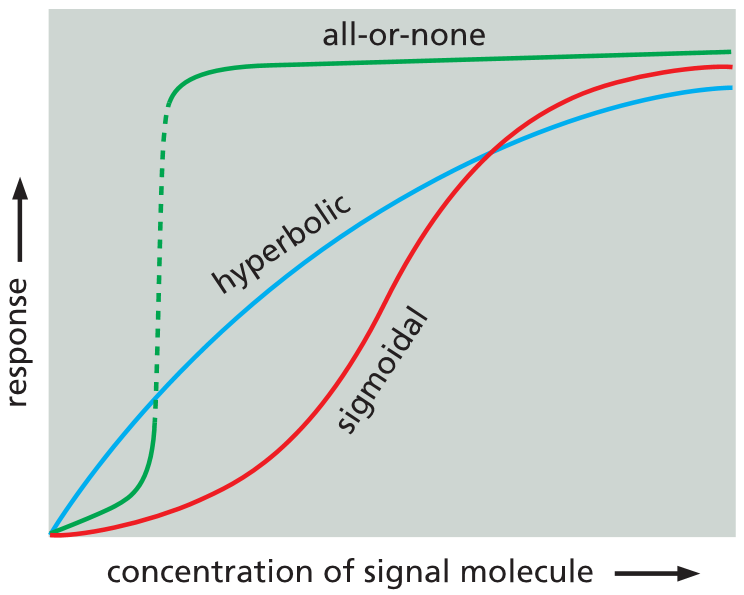
\includegraphics[width=0.5\textwidth]{resp_types}
	\caption{The three shapes a response tends to take in reaction to the signal. This is determined by how it is processed.}
\end{figure} 

When we analyze cells it is important to remember that we are taking an average response of all cells. While a hyperbolic response average is probably hyperbolic in all cells, what appears to be sigmoidal could actually be a all or nothing response with some cells firing and others doing nothing. Hence, it is important to analyze the individual cells too. Here is a visualization:
\begin{figure}[H]
	\centering
	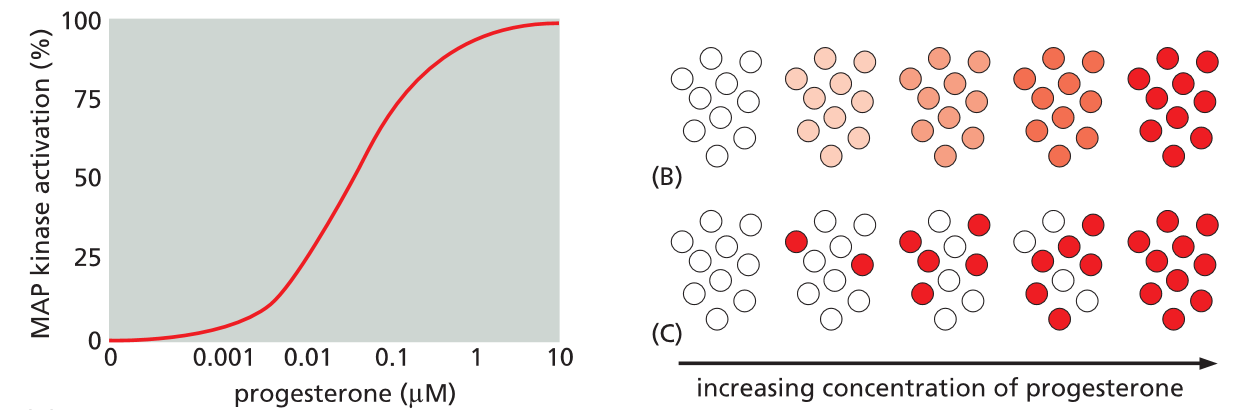
\includegraphics[width=0.5\textwidth]{resp_trick}
	\caption{What appears to be sigmoidal may actually be all or nothing.}
\end{figure} 




\section{Cell Signaling The World of G-proteins}

\subsection{The Components of a G-Protein Pathway}

Guanine nucleotide-binding proteins or \gls{GProteins} are a major type of cell-surface receptor. There are many different types of G proteins.

\subsubsection{G-Protein-Coupled Receptor or GPCR}

the G-protein-coupled-receptor (\gls{GPCR}) is the place the ligand attaches too. Then the GPCR will activate the G-protein. GPCR uses trimeric G-proteins.

\textbf{Structure}: A GPCR has seven transmembrane regions, composed of \textbf{7 alpha helices and 6 loops}. It has a N-terminal extracellular region and a C-terminal intracellular region. The alpha helices form a pocket for the ligand to bind. Depending on the size of the ligand GPCR will have a differently sized extracellular domain to accomadate for the ligand, while remaining specific. There are over 700 different GPCR in humans.

\begin{figure}[H]
	\centering
	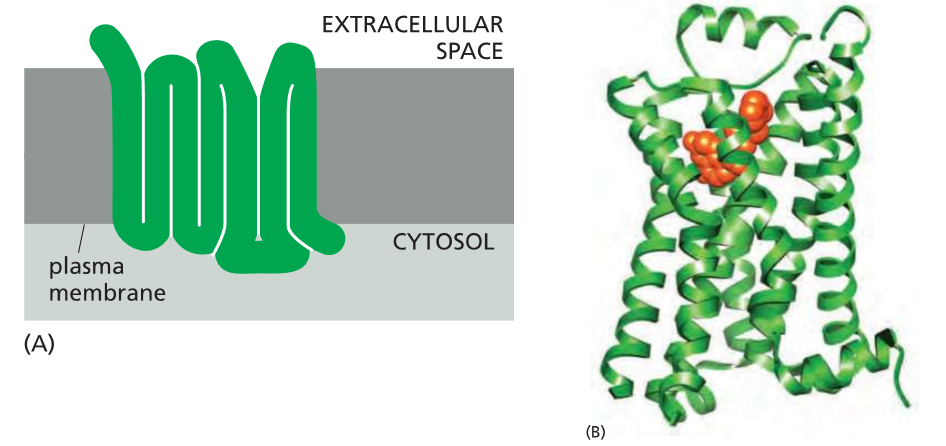
\includegraphics[width=0.45\textwidth]{GPCR}
	\caption{Simplified image of GPCR in membrane and its 3D structure.}
\end{figure}

\subsubsection{\gls{HeterotrimericGProtein}}

\begin{figure}[H]
	\centering
	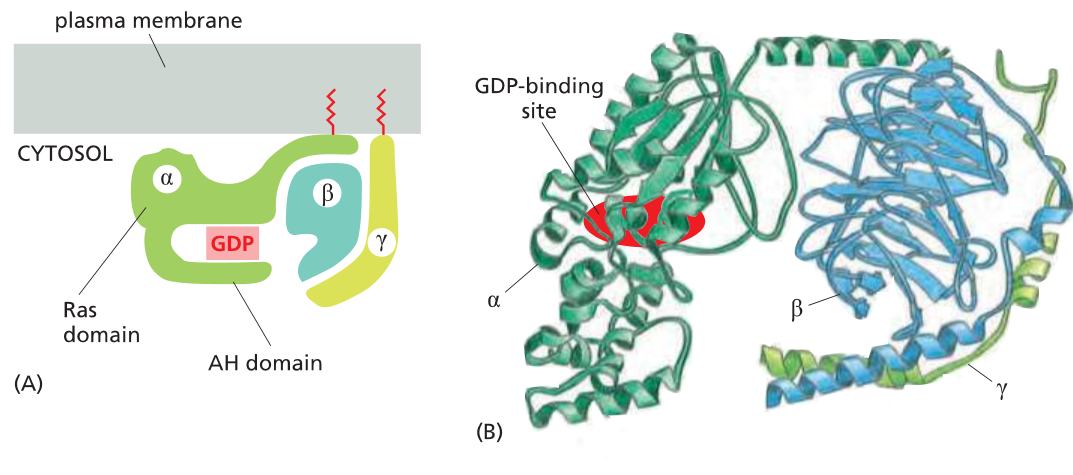
\includegraphics[width=0.45\textwidth]{G_structure}
	\caption{Simplified image of G-Protein in membrane and its 3D structure.}
\end{figure}

Some quick facts:
\begin{itemize}
	\item 3 proteins that make up the G-protein
	\item The G-proteins \gls{AlphaSubunit} is a \gls{GTPases}.
	\item GPCR uses trimeric G-proteins.
	\item at least 20 different alpha subunits exist.
	\item there are numerous different \gls{BetaComplex} and \gls{GammaComplex}, meaning we have quite a number of different G-proteins out there.
\end{itemize}

There are a bunch of different trimeric G-proteins, which are split into four major families, which all have different functions:
\begin{figure}[H]
	\centering
	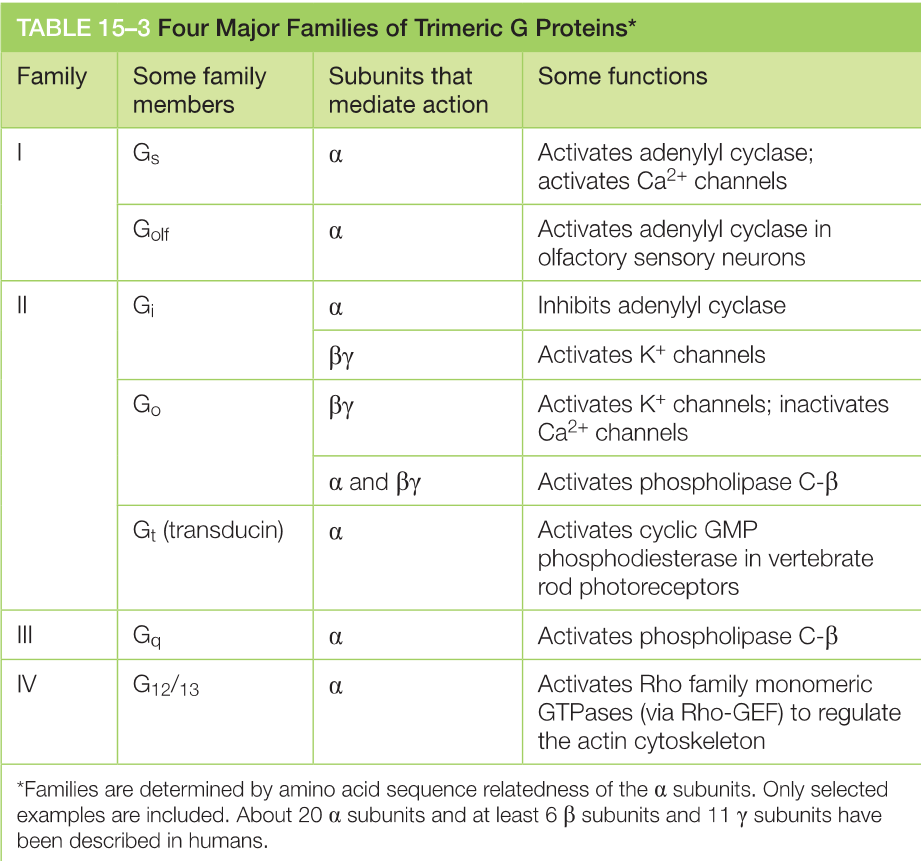
\includegraphics[width=0.45\textwidth]{G_families}
	\caption{Shows the four major families of trimeric G-proteins.}
\end{figure}

\textbf{Function}: The \gls{RasDomain} is part of the alpha subunit and is related to GTPases and provides a face for GDP/GTP to bind too. The \gls{AlphaHelix} domain binds it in place. Activation from a GPCR triggers the release of GDP from the alpha subunit followed by the binding of GTP
 
\subsubsection{Activation of G-Protein by GPCR}

Here is how GPCR activates a G-protein:
\begin{enumerate}
	\item An extracellular signal molecule binds to the GPCR molecule;
	\item The GPCR molecule changes conformation, which allows it to bind to the Ras domain of the G-protein;
	\item This alters the conformation of the alpha subunit, specifically the alpha helix subunit, releasing the GDP.
	\item The binding of GTP then promotes the closing of the subunit
	\item This triggers conformational changes causing the alpha subunit to dissociate from both the GPCR as well as the beta-gamma subunit.
	\item Both the alpha and the beta-gamma subunit then become active in downstream pathways.
	\item GPCR stays active as long as the ligand is bound to it, meaning it can activate many G-proteins.
\end{enumerate}

How an activated G-protein starts the \gls{DownstreamCascade}:
\begin{figure}[H]
	\centering
	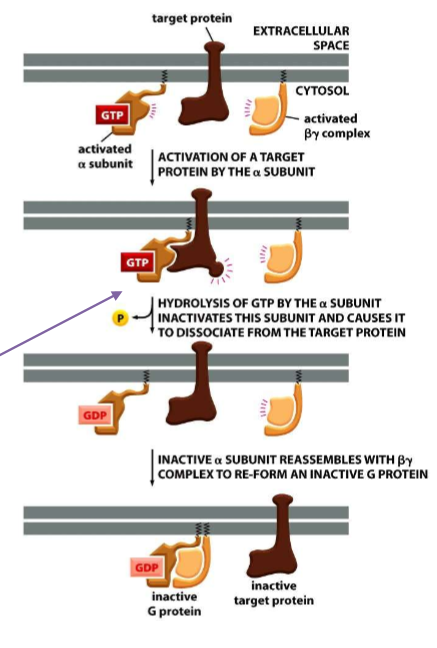
\includegraphics[width=0.45\textwidth]{G_usage}
	\caption{Once we have activated the G-protein and the subunits split, once they are used and the GTP is converted to GDP the inactive subunits merge back together and the cycle can start again.}
\end{figure}

The main \textbf{downstream targets}: 
\begin{itemize}
	\item \textbf{\gls{AdenylateCyclase}}, which in turn increases or decreases \textbf{\gls{cAMP}} (very common target);
	\item Channels;
	\item \textbf{\gls{PLC}}, which in turn generates IP3 and diacylglycerol.
\end{itemize}

\subsubsection{Stopping GPCR signaling}

The signalling of GPCR can be stopped through \textbf{\gls{GPCRKinases}} (\textbf{GRKs}) and \textbf{\gls{Arrestins}}, as they cause desensitization of the GPCR. The process:
\begin{enumerate}
	\item \textbf{\gls{NegativeFeedback}}: Activated GPCR stimulates GRKs which phosphorylate the GPCR on multiple sites. Note therefore GRK can only phosphorylate activated receptors.
	\item This allows the Arrestin to prevent the receptor from binding to its G-protein and directs the receptors endocytosis. 
\end{enumerate}
\begin{figure}[H]
	\centering
	\includegraphics[width=0.7\textwidth]{GRk}
	\caption{How GRK is a negative regulator, through negative feedback, for GPCR.} 
\end{figure}




\subsection{GPCR signaling through Cyclic AMP a.k.a. cAMP}
\subsubsection{cAMP}

Cyclic AMP a.k.a. \gls{cAMP} is a derivate of ATP. Two phosphates are replaced by a sugar bond, by enzyme \textbf{\gls{AdenylateCyclase}}. cAMP is a shortlived molecule which is "uncycled" to 5'-AMP, by enzyme\textbf{\gls{cAMPPhosphodiesterase}}. The fact the molecule is so shortlived makes it great as a signaling molecule.
\begin{figure}[H]
	\centering
	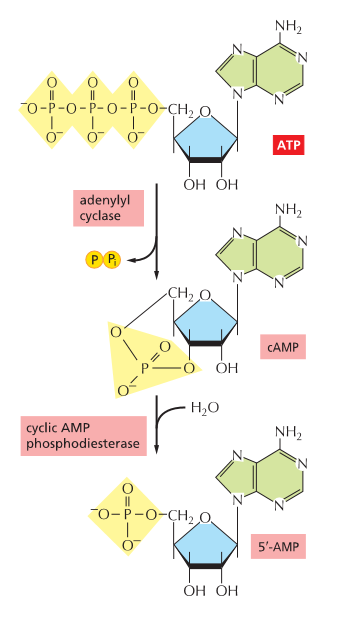
\includegraphics[width=0.45\textwidth]{cAMP_prod}
	\caption{The production of cAMP with the enzymes adenylyl cyclase and cAMP phosphodiesterase.}
\end{figure}

\begin{RemarkWithTitel}{cAMP jumping between cells}
	cAMP can be transported to other cells via \textbf{\gls{GAPJunctions}}.
\end{RemarkWithTitel}
\subsubsection{cAMP as a signaling molecule}

The pathway is as follows:

\begin{figure}[H]
	\centering
	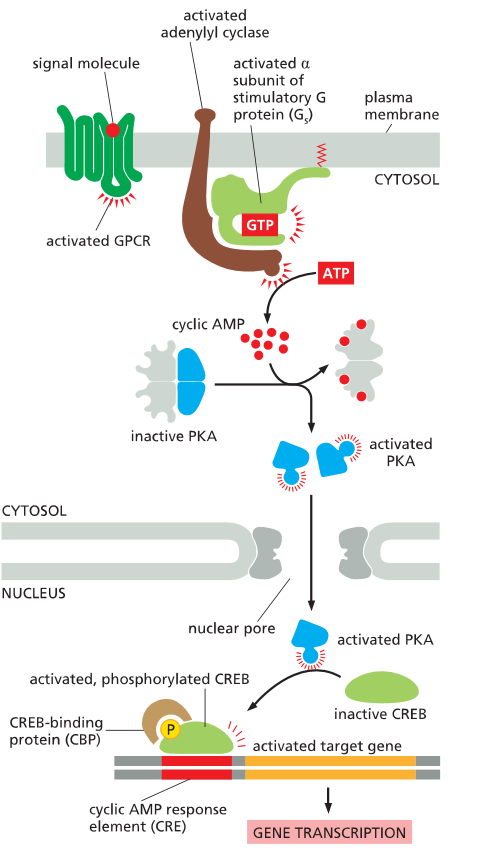
\includegraphics[width=0.45\textwidth]{cAMP_path}
	\caption{The production of cAMP with the enzymes adenylyl cyclase and cAMP phosphodiesterase.}
\end{figure}


\begin{enumerate}
	\item \textbf{Activation of GPCR}: GPCR gets activated, which in turn activates the adenylyl cyclase and the G-protein.
	\item \textbf{cAMP produced}: The activated adenylyl cyclase converts ATP into cAMP.
	\item \textbf{ Activation of \gls{PKA}}: The main role of cAMP is the activation cAMP-dependent \textbf{protein kinases} (PKAs). By binding to the regulatory subunits of the PKA tetramer induces a conformational change, which makes the regulatory subunits to dissociate from the catalytic subunits activating them. This release requires multiple cAMPs per regulatory unit. This means a lot of cAMP is required, as cAMP quickly decays, so we get a pretty sharp response.
	\begin{figure}[H]
		\centering
		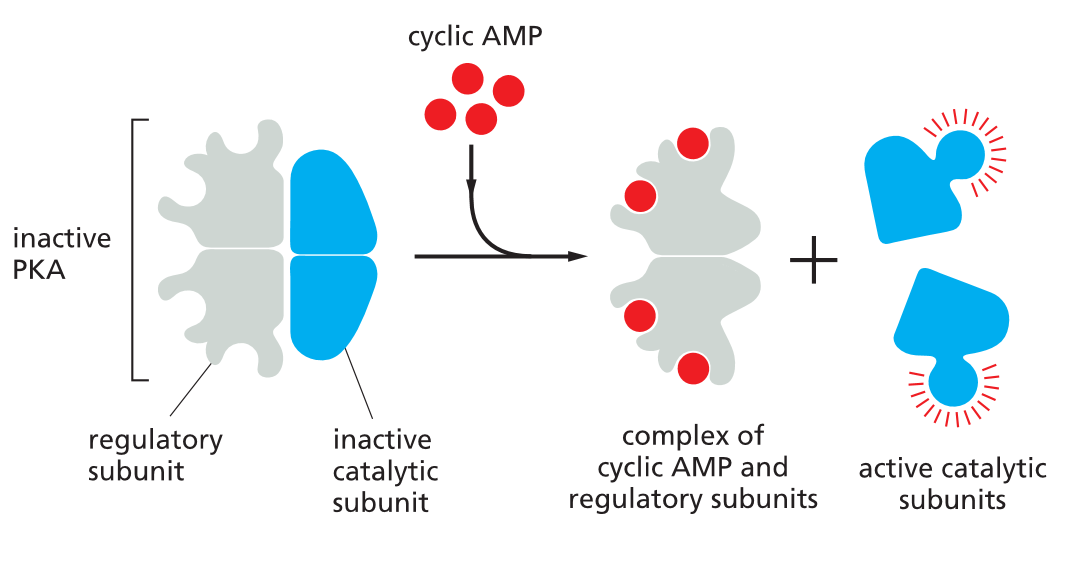
\includegraphics[width=0.6\textwidth]{cAMP_PKA}
		\caption{Shows the activation of PKAs by cAMP.}
	\end{figure}
	\item The active PKA is then translocated to the nucelus, where it activates a transcription factor \gls{CREB} (cAMP response binding protein) through phosphorylation.
	\item CREB interacts with CREB-binding protein and activates transciption on the cAMP response element.
\end{enumerate}

The activation of \gls{GPCR} by a ligand, say serotonin, increasing the signal strength 20fold in a matter of seconds. Depending on the cell and the ligand we will get very different cell responses. The PKA however will always be the same and it is the substrate of the PKA that changes. Hence we can receive so many different responses. Here are some examples with hormones:
\begin{figure}[H]
	\centering
	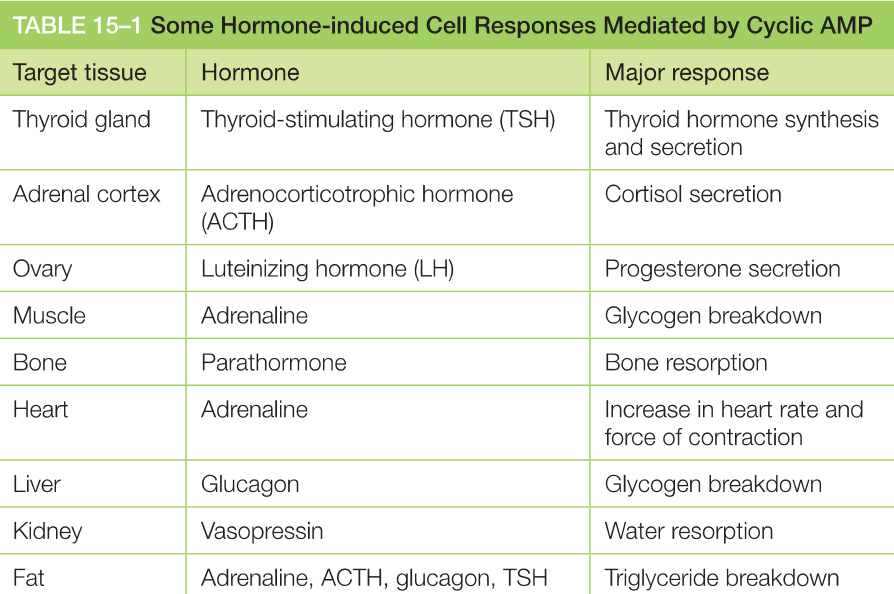
\includegraphics[width=0.45\textwidth]{cAMP_horm}
	\caption{The expression using different hormones in different cells. Vasopressin is also a "love" hormone, meanign that when you are in love GPCR is active}
\end{figure}

\subsubsection{cGMP}

Cyclic-Guanine-Mono-Phosphate or \textbf{\gls{cGMP}} is an alternative in the cAMP pathway. So, sometimes cGMP is activated by GPCR not cAMP. The only difference is the guanine instead of adenosine. The enzyme is called \textbf{\gls{GuanylateCyclase}}. 


\begin{figure}[H]
	\subfigure[The structure of cGMP, where the only difference to cAMP is the guanine for adenosine.]{
		\includegraphics[width=0.45\textwidth]{cGmp}
	}
	\subfigure[How the cell changes when light is received. Note that the signal sent to the brain is inversed of how a normal neuron is fired (channels close instead of open).]{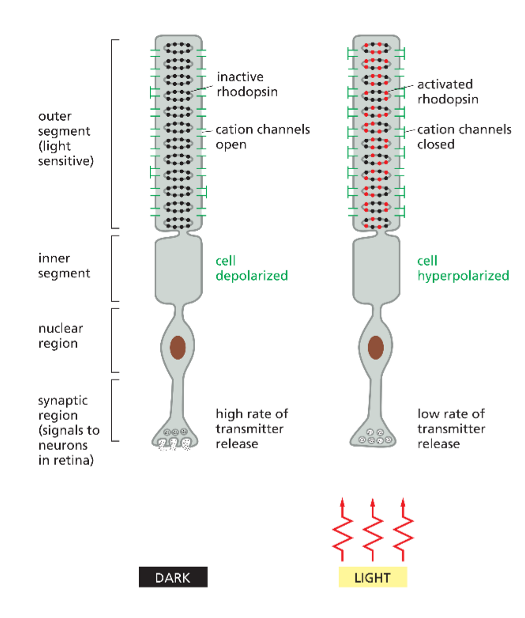
\includegraphics[width=0.45\textwidth]{cGMP_rhod}}
	\caption{cGMP}
	\label{fig:cGMP}
\end{figure}

\subsubsection{Case study with response to light}

The process of recognition is as follows (see fig:\ref{fig:cGMP}):
\begin{enumerate}
	\item a \textbf{\gls{Rhodopsin}} molecule absorbs a photon;
	\item 500 G-proteins molecules (\gls{Transducin}) are activated (signal is amplified);
	\item 500 \gls{cGMPPhosphodiesterase} molecules are activated;
	\item $10^{5}$ \gls{cGMP} are hydrolyzed (signal has been amplified);
	\item They block 250 cation channels;
	\item $10^{6} - 10^{7} Na^{+}$-ions per second are prevented from entering the cell for a period of around a second (signal has been amplified);
	\item The membrane potential is altered by 1mV, which in turn relays a signal to the brain. 
\end{enumerate}

\subsection{GPCR Signaling through phosphlipase C}
\label{sec:PLC}
Here are some example cell responses where GPCRs activate \gls{PLC}$\beta$
\begin{figure}[H]
	\centering
	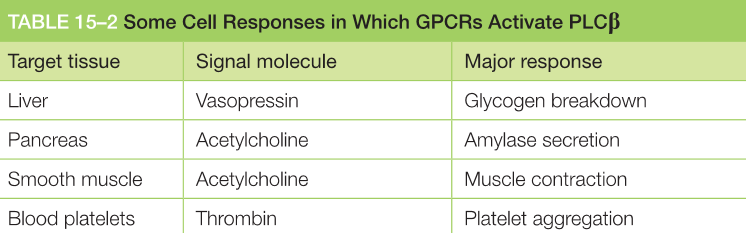
\includegraphics[width=0.6\textwidth]{PLC_ex}
	\caption{Some cell responses where GPCR activates PLC$\beta$, shoutout to Vasopressin for all the lovin'.}
\end{figure}

\subsubsection{Case Study: GPCRs activating Cytosolic Ca2+ and activating protein Kinase C}
\begin{figure}[H]
	\centering
	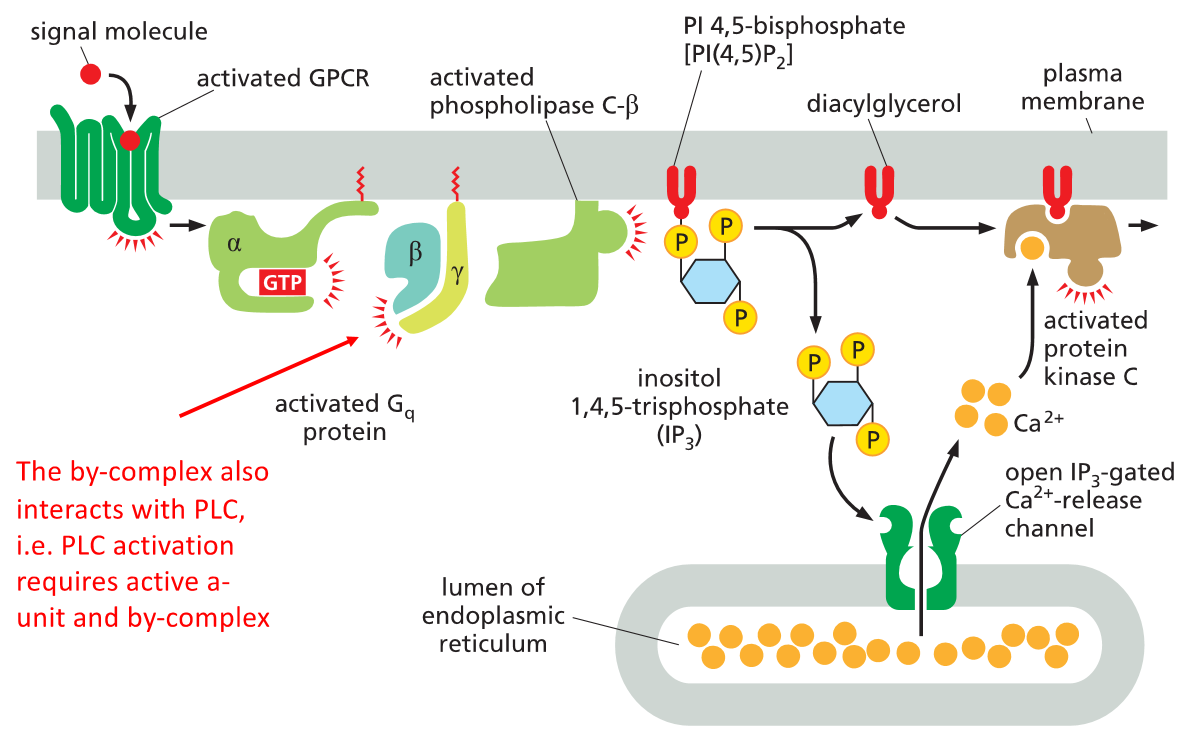
\includegraphics[width=0.6\textwidth]{PLC_Ca}
	\caption{Shows the pathway of GPCR activating Cytosolic \gls{Calcium}.}
\end{figure}
Rundown of the pathway:
\begin{enumerate}
	\item The GPCR activates the PLC$\beta$ via a G-protein called \gls{Gq}. The Gq Beta-gamma complex and the alpha-complex activates the PLC$\beta$. 
	\item PLC$\beta$ hydrolyzes \gls{PI}(4,5)P2, causing it to split into two messengers
	\item IP3 diffuses through the cytosol and releases Ca2+ from the ER by binding to the IP-gated Ca2+ channels.
	\item Then the diacyglycerol, \gls{DAG}, (other part of PI(4,5)P2), remaining in the membrane, together with the Ca2+ and \gls{Phosphatidylserine} activate the protein Kinase C (\gls{PKC}). Of the min. 10 forms of PKC at least 4 are activated by DAG.
\end{enumerate}

\subsubsection{Ca2+ feedback waves and oscillations}

The concentration of \gls{Calcium} plays a big role in activating or inactivating. So, giving itself positive or negative feedback. Here's how:
\begin{itemize}
	\item \textbf{Activation}: At low concentrations, Ca2+ goes to neighboring channels and activates them, causing the release of more Ca2+ and a wave like reaction across receptors (first couple pics). This means that the channels can stay active even without any IP3 being present.
	\item \textbf{Inactivation}: When Ca2+ is present at very high concentrations it inactivates the channels. That means that now we create a wave of inactivation.
	\item \textbf{\gls{Oscillation}}: In the continued presence of the ligand activator, or even without, this mix of feedback can cause oscillations in Ca2+ excretion.
\end{itemize}
\begin{figure}[H]
	\centering
	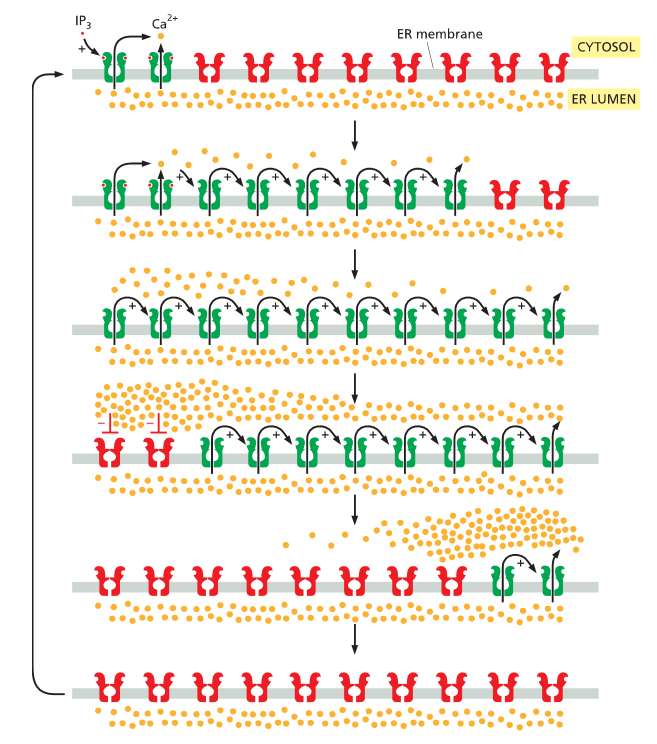
\includegraphics[width=0.45\textwidth]{Ca2_waves}
	\caption{Shows how Ca2+ influences the activity of its own channels}
\end{figure}

\subsubsection{How Ca2+ plays an important role in regulating and relaying signals}

\textbf{Ca2+ and \gls{Calmodulin}}: With the help of Ca2+/calmodulin, Ca2+ is able to bind to target proteins and with that relay the signal. The dumbbell shape of calmodulin and alpha-helix allows it to take on numerous different conformations.
\begin{figure}[H]
	\centering
	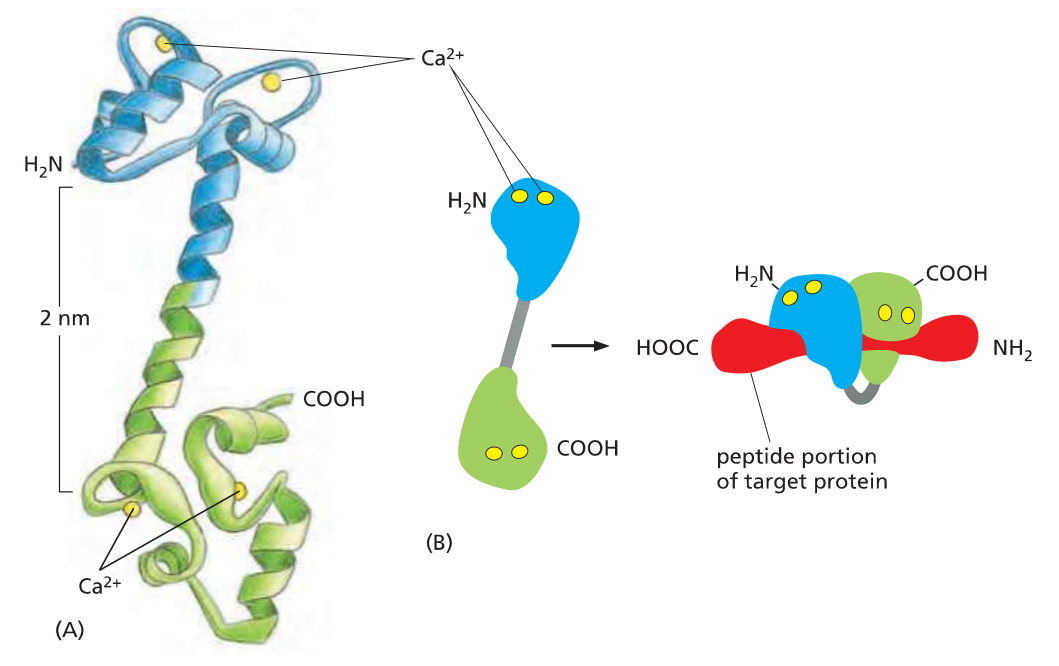
\includegraphics[width=0.45\textwidth]{Ca2_cal}
	\caption{On the left the structure of calmodulin and on the right an example of how it can bind to target proteins (this move is called the jackknife).}
\end{figure}

\textbf{CaM-Kinase II} is regulated by calmodulin. Here's how that runs down:
\begin{enumerate}
	\item 6 \gls{CaMKII} (green) form a ring. 
	\item The kinase domains pop in and out naturally.
	\item Calmodulin can bind the popped-out domain in place when it is bound to Ca2+
	\item Then that kinase domain gets \gls{Autophosphorylation}, making it active.
	\item In the continued presence of calmodulin it is even more active.
	\item Becomes inactive through dephosphorylation
	\item The more domains are active, the more active the enzyme as a whole.
\end{enumerate}
\begin{figure}[H]
	\centering
	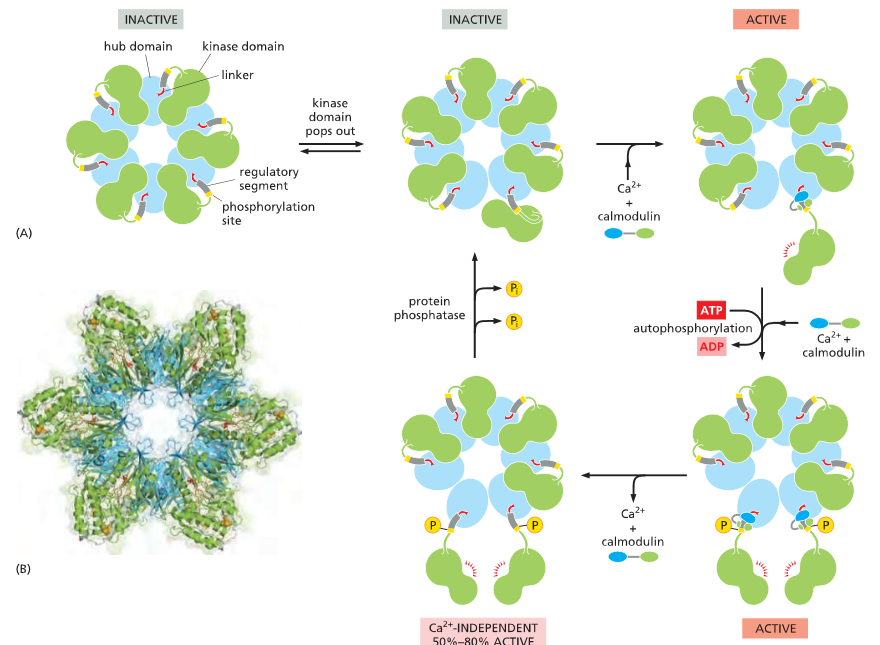
\includegraphics[width=0.7\textwidth]{Ca2_cam}
	\caption{Shows how Ca2+/calmodulin activate enzymes, in this case CaM-KII.}
\end{figure}

Depending on the frequency of the Ca2+ oscillations, the activity of the enzyme is influenced in major ways. The more frequent the oscillations the more the activity as a whole will rise. \\
For instance at low frequency the autophosphorylation induced by the Ca21/calmodulin binding does not maintain the enzyme's activity long enought for the enzyme to ramain active untile the next Ca21 spike arrives. At a higher spike frequencies, however, the enzyme fails to inactivate completely between the spikes, therefore its activity ratchets up with each spike.\\
Hence CaM-KII is a good mechanism of decoding the frequencies of oscillations in a cell. Here's a figure to visualize:
\begin{figure}[H]
	\centering
	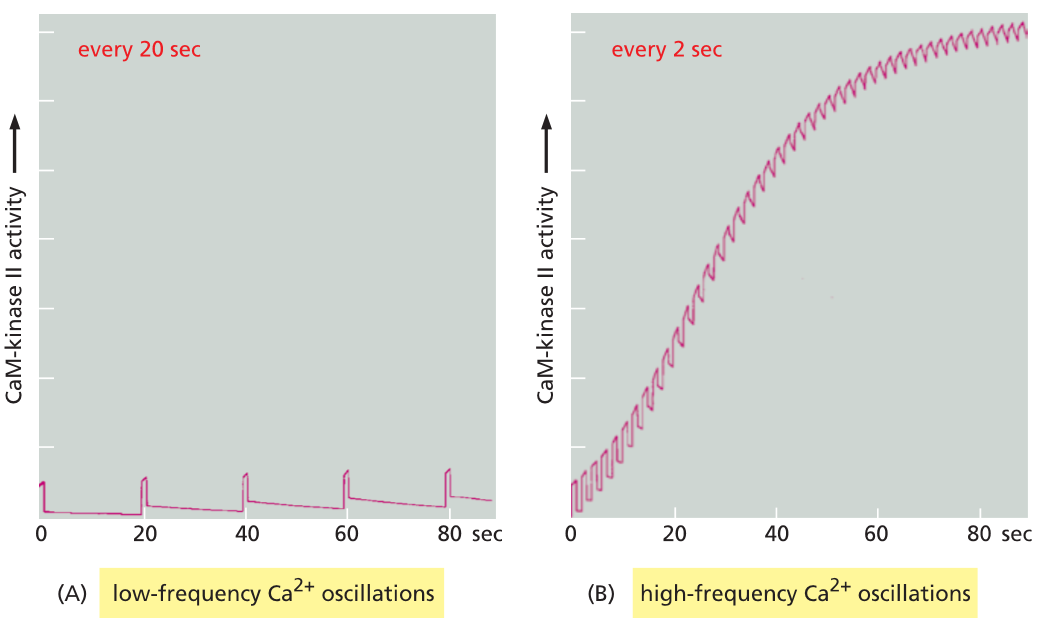
\includegraphics[width=0.45\textwidth]{Ca2_osc}
	\caption{How different frequencies of oscillations cause major differences in enzyme activity.}
\end{figure}





\section{Cell Signaling: Receptor Tyrosine Kinase a.k.a. RTKs}

Receptor Tyrosine Kinases are a large group, here are some of them:
\begin{figure}[H]
	\centering
	\includegraphics[width=0.6\textwidth]{RTk_ex}
	\caption{A bunch of different RTK groups}
\end{figure}

\textbf{\gls{RTK}} are connected by the fact that they all have an intracellular kinase domain which can phosphorylate a Tyrosine. The extracellular domain on the other hand is completely variable. the kinase region can also have a \textbf{\gls{kinaseinsertregion}} important for interactions with other proteins.

\begin{figure}[H]
	\centering
	\includegraphics[width=0.7\textwidth]{RTk_types}
	\caption{A bunch of different RTK types, with the core features.}
\end{figure}

\subsection{Activation of RTKs by \gls{Dimerization}}

\begin{enumerate}
	\item Two RTKs are initially inactive until some type of ligand arrives to bring them together.
	\item In this proximity the RTKs \textbf{dimerize} and make an initial Tyrosine \textbf{\gls{Autophosphorylation}}.
	\item Once the first phosphorylation has happened that initiates \gls{Transphosphorylation} of several Tyrosines.
	\item \gls{Phosphotyrosin} sites recruit and/or activate downstream signaling proteins.
\end{enumerate}
\begin{figure}[H]
	\centering
	\includegraphics[height=0.3\textwidth]{RTk_act}
	\caption{Activation of a RTK dimer}
\end{figure}

\subsection{An exception to the rule: Activation of \gls{EGFKinase}}

Compared to the regular activation the kinase domains are not both auto-phosphorylated to be activated. We still have two identical domains, but one takes on the role of activator, while the other is the receiver.

\begin{enumerate}
	\item Both domains are activated through EGF.
	\item Then the activator pushes on the receiver, causing a conformational change in the receiver domain, which makes it active. 
	\item The receiver Kinase domain then phosphorylates the tyrosines on both receptors.
\end{enumerate}

\begin{figure}[H]
	\centering
	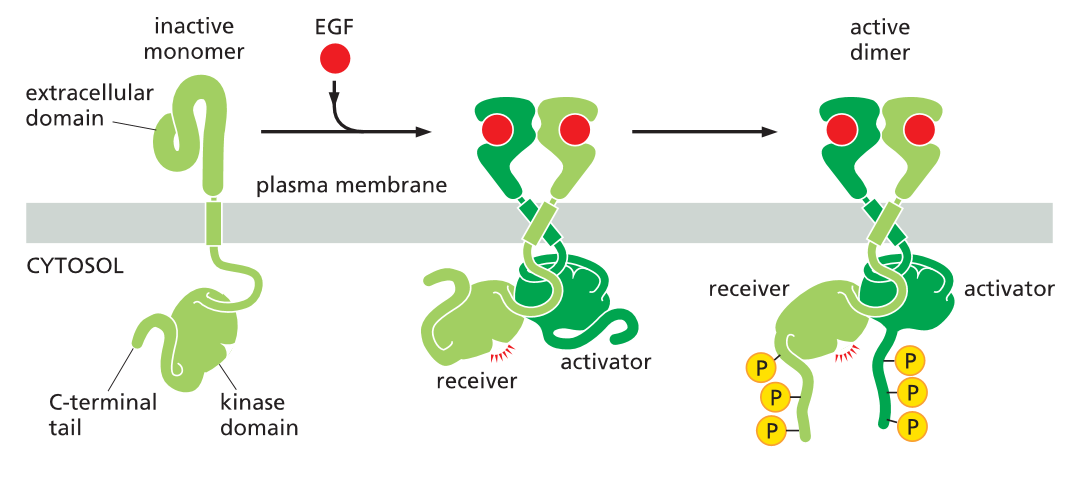
\includegraphics[width=0.7\linewidth]{egf_path}
	\caption{The activation of a EGF receptor kinase.}
	\label{fig:egfpath}
\end{figure}


\begin{RemarkWithTitel}{Cancerous EGF Kinase}
	If the receiver domain mutates in such a way that it is constitutively active, then \gls{RasMPK} and \gls{PI3K} are also always activated resulting in uncontrolled cell growth.
\end{RemarkWithTitel}


\subsection{Tyrosine Kinase Associated Signaling}
\subsubsection{JAK-SAT}

\textbf{\gls{JAK}} stands for JANUS Kinases, which are part of\textbf{\gls{kinasecytokinereceptors}}. 

They work very similar to a regular RTK, with the JAK-STAT being cytokine receptors:
\begin{enumerate}
	\item once the ligand connects the cytokine receptors get together and become active.
	\item The activation of the JAKs, which are associated with the receptors, happens through cross phosphorylation of each other.
	\item Then the JAKs phosphorylate the receptors at a Tyrosine, on the receptor.
	\item Said phospho-Tyrosine can then recruit \textbf{\gls{STAT}} proteins.
	\item Once they have docked they get phosphorylated by the JAKs, making them active.
	\item Then they enter the cytosol and translocate to the nucleus.
	\item In the nucleus they associate with a complex and activate transcription.
\end{enumerate}

\begin{figure}[H]
	\centering
	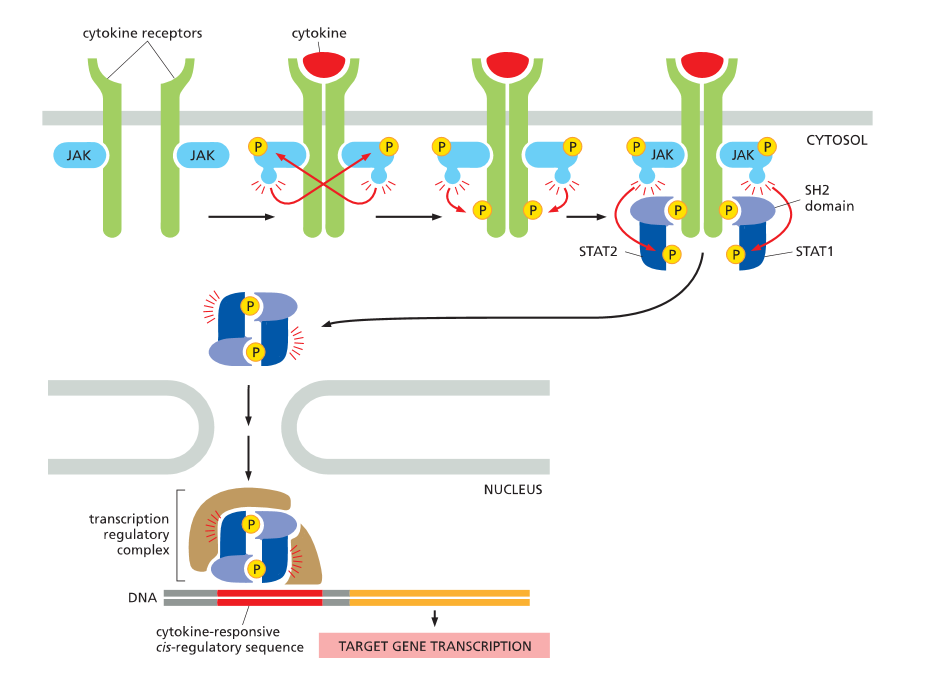
\includegraphics[width=0.7\linewidth]{Jak_mech}
	\caption{The JAK-SAT pathway. The exact details on the complex for transcription are beyond this course.}
\end{figure}

There are 4 different JAKs and 7 STATs, which are very important and especially known for immune responses. They are the following:
\begin{itemize}
	\item JANUS Kinases:
	\begin{enumerate}
		\item JAK1
		\item JAK2
		\item JAK3
		\item TYK2 (you thought this was about to say JAK 4 didn't you)
	\end{enumerate}
	\item STATS
	\begin{enumerate}
		\item STAT1
		\item STAT2
		\item STAT3
		\item STAT4
		\item STAT5a
		\item STAT5b (gotcha again, not 6 just yet)
		\item STAT6
	\end{enumerate}
\end{itemize}

It is a very diversely used pathway, which over 128 extracellular signaling proteins and their receptors using JAK-STAT. Here are some signaling proteins:

\begin{figure}[H]
	\centering
	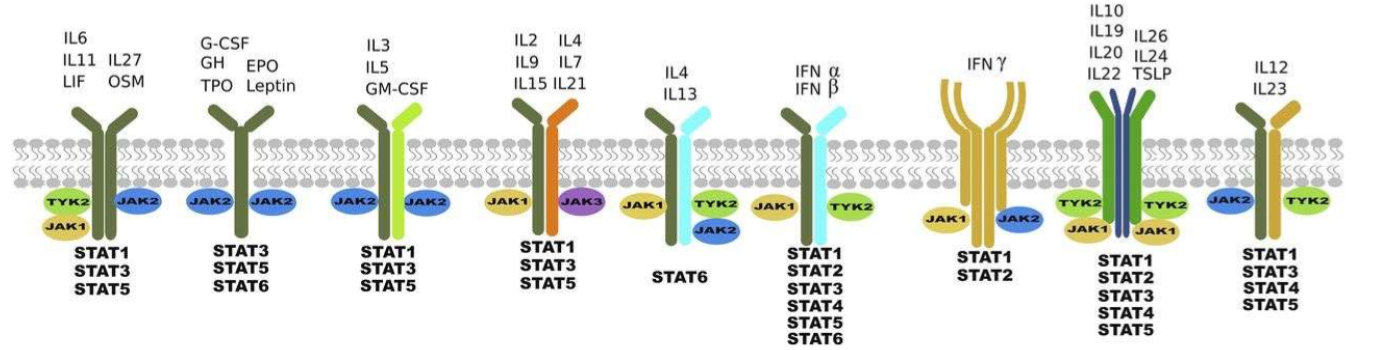
\includegraphics[width=0.7\linewidth]{Jak_sig}
	\caption{A bucnh of signaling proteins which use JAK-STAT.}
\end{figure}


As per usual here a bunch of different JAK-STATs in the body:
\begin{figure}[H]
	\centering
	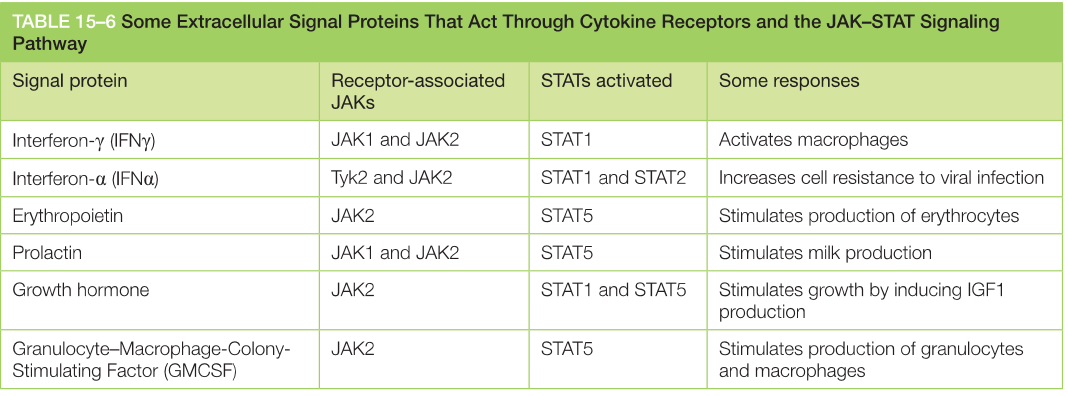
\includegraphics[width=0.7\linewidth]{Jak_ex}
	\caption{A bunch of different JAK-STATS in humans}
\end{figure}

Also JAK-STAT and \gls{FGFR} signaling inhibition can restore sensitivity to anti-hormonal drugs in prostate cancer [Editor's note: I have no idea how important this is, guessing this is to some degree his research or something.] 


\subsubsection{TGF Beta Signaling}
While Karthaus doesn't put it in the tyro-kinase associated box, I feel like it fits, so we putting it here :)

 
\begin{figure}[H]
	\centering
	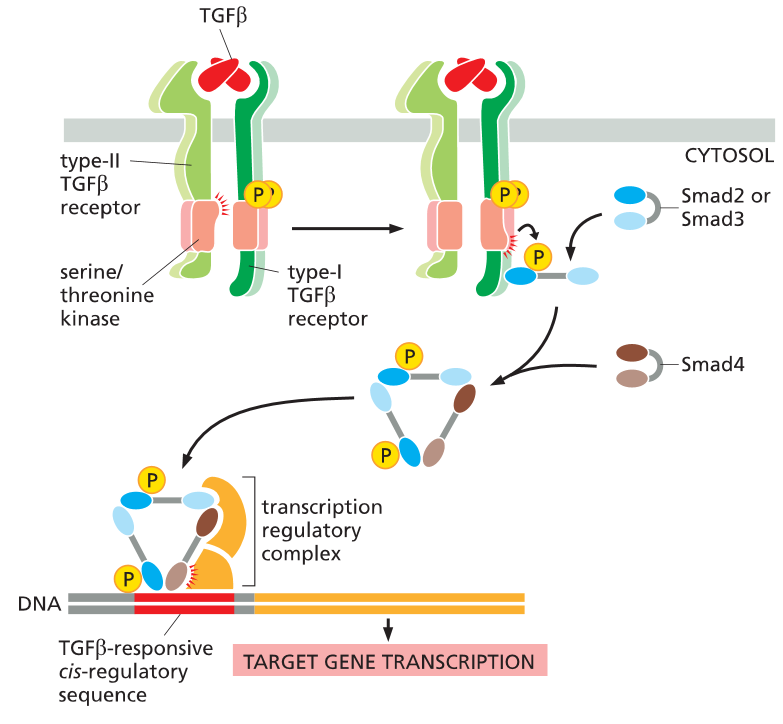
\includegraphics[width=0.7\linewidth]{TGF_path}
	\caption{The TGF-beta pathway, using Smad}
\end{figure}


\begin{enumerate}
	\item The \gls{TGFbeta} dimer promotes the assembly of a tetrameric receptor complex of TGF$\beta$'s containing two copies of the \gls{typeIreceptor} and \gls{typeIIreceptor}.
	\item type-II receptors phosphorylate type-I receptors, which activate their kinase activity.
	\item type-I receptors then activate R-\gls{Smad}, such as Smad2 or Smad3.
	\item This leads p-Smads to open up and be exposed to dimerization of the phosphorylated surface
	\item This leads to trimerization, with the co-Smad, Smad 4. 
	\item This Smad complex then enters the nucleus, and joins an even bigger transcription complex
\end{enumerate}





\section{RTK and G-Protein: Downstream and Similarities}


\subsection{Checking out how GPCRs and RTKs are intertwined}
\begin{figure}[H]
	\centering
	\includegraphics[width=0.5\linewidth]{GPCR_RTK}
	\caption{Compares the pathways caused by GPCRs and RTKs, also shows which are shared. All of them end with a Kinase, which then causes a reaction chain downstream}
\end{figure}

Both GPCR and RTK have a \gls{PLC} enzyme, called beta and gamma respectively. The effect is very similar.

\subsection{Binding to the Receptor}

\begin{figure}[H]
	\centering
	\includegraphics[width=0.7\linewidth]{pdgf}
	\caption{Phospho-tyrosine on PDGF receptors being docking-sites for proteins containing SH2 or PTB domains.}
	\label{fig:pdgf}
\end{figure}


The phospho-tyrosines are docking sites for proteins containing:
\begin{enumerate}
	\item \gls{SrcHomology(SH)}, \gls{protooncogene}
	\item \gls{PhosphotyrosineBinding(PTB)}, \gls{protooncogene}
	\item \gls{PLC} 
\end{enumerate}

Because of the multitude of phospho-tyrosines many different proteins, and consequently different pathways, can interact with the receptors.

\subsubsection{Ras signaling}

\gls{Ras} is essentialy a \textbf{monomeric GTPase}. Ras is \textbf{anchored to the membrane} through a lipid modification. For a refresher on how GTP can be regualted please refer to Section \ref{sec:GTP}.

Here are some groups:
\begin{figure}[H]
	\centering
	\subfigure[Ras groups in our body.]{
		\includegraphics[width=0.4\textwidth]{Ras_ex}
	}
	\subfigure[The pathway for Ras.]
	{\includegraphics[width=0.55\textwidth]{ras_sig}}
	
\end{figure}

\textbf{Activation of Ras by an  RTk}: 
\begin{enumerate}
	\item Adaptor protein \gls{Grb2} docks to RTk with \gls{SrcHomology(SH)}
	\item Ras-GEF then interacts with Grb2
	\item Ras-GEF then exchanges the GDP for a GTP
	\item Ras is activated.
\end{enumerate}

\begin{RemarkWithTitel}{Detecting Ras activity}
	We use \gls{FRET} (Fluorescence resonance energy  transfer), by attaching a yellow fluorescent protein (YFP) to the gene of Ras. Then we add a red fluorescent dye to GTP. That way when no GTP is there (Ras inactive), it emits yellow light, but when GTP is attached to the Ras (active) red light is emitted.
\end{RemarkWithTitel}


\begin{figure}[H]
	\centering
	\includegraphics[height=0.3\textwidth]{Ras_FRET}
	\caption{How FRET can be used to detect the activity of Ras.}
\end{figure}

\textbf{Case study: \gls{MAP} kinase module} is a module activated by \gls{Ras}. This is done the following way: Ras activates \gls{Raf} to the membrane, which in turn activates \gls{MEK}, which in turn activates \gls{Erk}, which phosphorylates a bunch of downstream proteins, such as further kinases, and transciption regulators. The resulting activations cause complex changes in the cell.
\begin{figure}[H]
	\centering
	\includegraphics[height=0.4\textwidth]{Ras_MAP}
	\caption{How the MAP kinase module is activated by Ras.}
\end{figure}

\textbf{How cancer changes Ras}: By changing certain amino acids (G12, G13, Q61), the mutants show impaired GTPase activity, leading to a gain-of-function. So, the GAP proteins no longer work as well. Of the three types of famous Ras (K,H,N-Ras) it seems mostly the mutant K-Ras is found in cancers. Mutant Ras probably important in the initiation of tumors. GAP is a \gls{TumorSuppressor}, EGF-R a \gls{protooncogene}.
\begin{figure}[H]
	\centering
	\includegraphics[height=0.3\textwidth]{Ras_canc}
	\caption{Showing how mutating the GAP messes with the regulation of Ras.}
\end{figure}

\subsubsection{PI3K signaling}

The PI3-Kinase phosphorylates the 3-carbon of a given \gls{PI} molecule (can already be phosphorylated at other carbons or not). This then creates docking sites for downstream proteins, prominently \gls{AKT}. In an alternative pathway the PI can also be activated by \gls{PLC} causing it to go down the PLC pathway (see section \ref{sec:PLC}). However, these are two independent pathways, even if the starting substrate PI is the same!


\begin{figure}[H]
	\centering
	\includegraphics[height=0.3\linewidth]{PI3_phos}
	\caption{Phosphorylation of the 3-carbon activates the PI.}
\end{figure}

\textbf{PI 3-Kinase activates \gls{AKT}}:
\begin{enumerate}
	\item \gls{PI3K} is recruited by RTK
	\item PI3K creates docking sites on the PI where proteins with a PH domain can dock.
	\item \gls{PDK1} and \gls{mTORC2} activate \gls{AKT} a.k.a. Protein Kinase B by phosphorylation at two different sites, allowing p-AKT to disassociate from the membrane.
	\item p-AKT activates many cellular programs including cell growth and anti-apostosis (hinting that cancer may be interested here).
\end{enumerate}


\textbf{Negative regulation}: Phosphatase \gls{PTEN} removes phosphate from PI(3,4,5)P3, making it a negative regulator of the PI3K. \\

The fig: \ref{fig:PI3K} below shows on the left the entire pathway which promotes cell growth. The one on the left shows how the chain on the left continues leading to cell growth. The \gls{MAP} kinase can also go down the pathway on the right, meaning bot can promote cell growth.
\begin{figure}[H]
	\centering
	\subfigure[cell growth whole pathway]{
		\includegraphics[width=0.65\textwidth]{PI3_surv}
	}
	\hfill
	% Second subfigure
	\subfigure[cell growth comparison through the activation of mTORC1 by PI3K]{
		\includegraphics[width=0.3\textwidth]{PI3_comp}
	}
	\caption{Note: (a) mTORC2 is in action, activating ATK, while in (b) \gls{mTORC1} is in action, about controlling protein synthesis, growth, and metabolism (further downstream of ATK).}
	\label{fig:PI3K}
\end{figure}


\subsection{EGF Receptors in cancer}

In cancer \gls{EGFR} can become over-activated, making it a \gls{protooncogene}.

\begin{figure}[H]
	\centering
	\subfigure[Different ways EGFR can become over expressed in cancer]{
	\includegraphics[width=0.4\linewidth]{EGF_canc}
	}
	\subfigure[Showing the options of both missense and frame-keeping deletions, found through Sanger Sequencing.]{
		\includegraphics[width=0.4\linewidth]{EGF_muta}
	}
	\caption{}
\end{figure}

Mutations in cancer occur at the kinase domain of the receptor, leading to the domain being permanently active. Thus Ras-MAP Kinase and PI3K are always active, leading to uncontrolled cell growth a.k.a. cancer. These mutations will be deletions which keep the reading frame or missense mutations:
\begin{figure}[H]
	\centering
	
	\caption{}
\end{figure}

Inhibitors can target always active EGFR. Through this some pathways are now slowed down, leading to more normalized cell growth.


\section{Cell Signaling: Alternative Signaling}
\subsection{Signaling with Regulated Proteolysis}
The namesake for all these beauties comes from how the fruit fly looked when we fucked it up. Details at the start of each section.


\subsubsection{Notch}
\gls{Notch} = V-shaped indentation in the wing.

The idea here is that instead of having the receptor cause a phosphorylation or similar, we cleave the receptor so that the intracellular part becomes the downstream signal, entering the nucleus. Here is the detailed process, oriented aroud the red numbered arrows in the picture:

\begin{enumerate}
	\item First \gls{ProteolyticCleavage} (red arrow 1): inside the trans Golgi network NOTCH is cut to become a mature version where the two parts are connected noncovalently.
	\item these parts then migrate to the cell membrane. 
	\item Once the the Notch complex binds to the \gls{Delta}, through its repeating EGF regions on a neighboring cell, the two parts are split by endocytosis (red arrow 3).
	\item This split then exposes the cleavage site (red arrow 3) to make the cut, allowing the \gls{Notchtail} (a.k.a. notch intracellular domain a.k.a. NICD) to migrate the nucleus.
	\item the tail binds to \gls{Rbpsuh} protein, which then coverts from a repressor to an activator. 
\end{enumerate}

\begin{figure}[H]
	\centering
	\includegraphics[width=0.7\linewidth]{Notch_path}
	\caption{The Notch pathway, note that red arrows are cleavage sites.}
\end{figure}

\begin{DefWithTitle}{\gls{LateralInhibition} in Notch}
	 Notch is contact-dependent and not autocrine. This allows for one cell to become excited and in the process inhibiting the neighboring one, which is called lateral inhibition. 
\end{DefWithTitle}

Looking at the example of neural cell development. Initially all \gls{epithelialcells} want to become neural cells, however we don't want that many. So, instead if a \textbf{cell expresses \gls{Delta} than the neighboring ones know not to become a neural cell anymore}. Since, they all want to be neural cells though a competition starts to appear of who can produce the most delta ligands and the winner becomes the neural cell.

\begin{figure}[H]
	\centering
	\includegraphics[width=0.4\linewidth]{Notch_neural}
	\caption{Case study of Notch, showing how Notch and Delta help in cell development.}
\end{figure}



\subsubsection{WNT}
\gls{Wnt} = Wingless (WG) + Integration (t).

\textbf{Wnt is a special secreted ligand}, that through a bunch of lipid modifications, \textbf{associates to the plasma membrane} and doesn't travel very far. That means that the spread of Wnt is very limited to the neighboring cells.

Looking at the Wnt ligand pathway: the broad idea is that we want to stop the degradation of the anti-repressor. \\

Here are the details, first in the absence of the Wnt ligand:
\begin{enumerate}
	\item \gls{BetaCatenin} interacts with degradation complex.
	\item In this complex it is phosphorylated first by \gls{CK1}, then \gls{GSK3}, triggering its ubiquitylation and then degraded.
	\item The degraded form prohibits it from binding to  \gls{LEF1}/TCF, meaning it can't kick out the repressor \gls{Groucho}.
\end{enumerate}

Now, in the presence of the Wnt ligand:
\begin{enumerate}
	\item Wnt binds to frizzled and LRP, clustering the two co-receptors together
	\item The tail of LRP is phosphorylated by GSK3 and then CK1. Further \gls{Disheveled} is recruited to the \gls{frizzled} site. The exact role of disheveled isn't known.
	\item The \gls{Axin}, of the degradation complex, is then recruited by the disheveled and then bound to the phosphorylated LRP.
	\item This results in the disassembly of the degradation complex.
	\item This means the $\beta$-catenin stays stable, attaches to the LEF1/TCF and kicks out Groucho.
\end{enumerate}

\begin{figure}[H]
	\centering
	\includegraphics[width=0.7\linewidth]{Wnt_path}
	\caption{The Wnt pathway, on the left without Wnt, leading to no expression, while on the right it has Wnt, meaning the gene is expressed.}
\end{figure}


\subsubsection{Hedgehog}
\gls{Hedgehog} = Larva looked like a hedgehog.

The game is all about \gls{CubitusInterruptus} (Ci). Without Hedgehog it get cleaved to a repressor, with Hedgehog it is an activator. \\

Here is what happens when we have no hedgehog:
\begin{enumerate}
	\item Through the absence of Hedgehog, \gls{Patched} is allowed to exist, which means it inhibits \gls{Smoothened}. 
	\item The lack of Smoothened which causes Ci to be caught in a degradation complex.
	\item This degradation complex includes a Fused kinase and a scaffold protein \gls{Costal2}. Costal2 recruits three other kinases (PKA, GSK3, CK1), which phosphorylate Ci. 
	\item That P-Ci is ubiquitylated and cleaved in proteasomes.
	\item the cleaved Ci then forms a repressor and moves to the nucleus to do just that.
\end{enumerate}

Now, when we have hedgehog:
\begin{enumerate}
	\item Hedgehog binding to \gls{iHog} as \gls{Patched} is removed and degraded, stopping the inhibition of Smoothened. 
	\item Smoothened is then phosphorylated by PKA and CK1 and translocated to the plasma membrane.
	\item There it recruits Fused, Costal2, which are forced to let go the Ci they were holding on to.
	\item The Ci enters the nucleus in its complete form and activates the hedgehog genes.
\end{enumerate}

\begin{figure}[H]
	\centering
	\includegraphics[width=0.8\linewidth]{Hedge_path}
	\caption{Shows the pathway of Hedgehog; on the left without Hedgehog, meaning gene repression; and on the right with Hedgehog and activation.}
\end{figure}

\subsubsection{\gls{NFKB} pathway}

Core concept - \gls{NegativeFeedback} Loop: What this causes is that the moment a gene is expressed it immediately inhibits its own transcription. That leads to a short expression, which is quickly blocked out.

\begin{RemarkWithTitel}{Application to NFkb}
	Activated NFkB increases expression of the IKB$\alpha$ gene, and IKB$\alpha$ then binds to NFkB	and inactivates it, thereby shutting of the response. If the initial activating signal persists, then additional cycles of NFkB act on and inactivation may follow.
\end{RemarkWithTitel}


\begin{figure}[H]
	\centering
	\includegraphics[width=0.7\linewidth]{NF_theo}
	\caption{The left shows the idea behind a negative feedback. The middle has a short TNF pulse, while the one on the right has a sustained one.}
\end{figure}

For the short TNF pulse: Gene A gets its transcription turned on by this while gene B does not. For the prolonged TNF exposure: gene B will also be transcribed. Why gene B needs that prolonged exposure isn't understood. Note that due to the negative feedback loop we get an oscillation of TNF until it finds the right concentration steady state with the gene. \\


NF-kB can be activated by many signals, a lot of them being \textbf{inflammatory signals} (infections, Bacteria, and immune cells secreting signals). \\

Now an example of the \gls{NFKB} pathway, activated by \gls{TNF}$\alpha$:
\begin{enumerate}
	\item TNF$\alpha$ is a trimer, as are its receptors. The binding of TNF$\alpha$ causes a rearrangement of the clustered tails of the receptors.
	\item These tails can now recruit a bunch of signaling prteins.
	\item This in turn activates the protein kinase which activates IkB kinase kinase (IKK). IKK is a heterotrimer composed of three subunits (\gls{IKKalpha} and \gls{IKKbeta} (catalytic subunits), and \gls{NEMO}(regulatory subunit)).
	\item IKK$\beta$ then phosphorylates two serine of IkB, which marks it for ubiquitylation and consequent degradation.
	\item The released NFkB translocates to into the nucleus, where it with co-activators stimulates transcription.
\end{enumerate}

\begin{figure}[H]
	\centering
	\includegraphics[width=0.7\linewidth]{NF_path}
	\caption{This shows the NFkB pathway.}
\end{figure}

In cells lacking NEMO, TNF triggers cell death.

\subsection{Nuclear Receptor Signaling}

Some signaling molecules can bind to intracellular molecules. This means they need to get through the membrane, so they got to be lipophillic. \textbf{\gls{Cholesterol} is kinda the God of precursors}, as its already in the membrane so must be popular. However, most of the signaling molecules will be more hydrophilic than cholesterol making them better for exiting membranes and transport throughout body.

The signaling with these molecules is incredibly simple. A dimer molecule comes in, reaches the nucleus and
\begin{itemize}
	\item changes the factors to activate gene expression. In the this process the receptors are already on the gene. This binding can also kick out inhibitors and often binds further activators.
	\item changes the factors to repress gene expression. This really is really just the same thing but opposite: activators are cleared out and repressor recruited. 
\end{itemize}

\begin{figure}[H]
	\centering
	\includegraphics[width=0.5\linewidth]{Nuc_act}
	\caption{How nuclear receptors attach right to the DNA, at the repressor (not shown) or activator site}
\end{figure}

Depending on the cell we will get completely different reactions and gene expressions.

\begin{RemarkWithTitel}{Use study - Prostate Cancer:}
	In prostate cancer, \gls{androgen} activate the \gls{androgenreceptor} (AR), which then turns on genes that support tumor growth and survival. In some therapeutic or experimental contexts, researchers can design genes controlled by androgen-responsive promoters so that their expression is turned on in the presence of androgen.
\end{RemarkWithTitel}

\begin{figure}[H]
	\centering
	\includegraphics[width=0.7\linewidth]{Nuc_foff}
	\caption{Yh I'm done with this, this is an example of Androgen being used to reprogram prostate cancer.}
\end{figure}


\end{document}